\documentclass[a4paper]{article}

\setlength{\parindent}{0pt}
\setlength{\parskip}{1em}

\pagestyle{headings}

\usepackage{amssymb}
\usepackage{amsmath}
\usepackage{amsthm}
\usepackage{mathtools}
\usepackage{graphicx}
\usepackage{hyperref}
\usepackage{color}
\usepackage{microtype}
\usepackage{tikz}
\usepackage{pgfplots}
\usepackage{pgfplotstable}

\newcommand{\N}{\mathbb{N}}
\newcommand{\Q}{\mathbb{Q}}
\newcommand{\Z}{\mathbb{Z}}
\newcommand{\R}{\mathbb{R}}
\newcommand{\C}{\mathbb{C}}
\newcommand{\D}{\mathcal{D}}
\renewcommand{\S}{\mathcal{S}}
\renewcommand{\P}{\mathbb{P}}
\newcommand{\F}{\mathbb{F}}
\newcommand{\E}{\mathbb{E}}
\newcommand{\bra}{\langle}
\newcommand{\ket}{\rangle}


\graphicspath{{Image/}}

\hypersetup{
    colorlinks=true,
    linktoc=all,
    linkcolor=blue
}

\theoremstyle{definition}
\newtheorem*{axiom}{Axiom}
\newtheorem*{claim}{Claim}
\newtheorem*{conv}{Convention}
\newtheorem*{coro}{Corollary}
\newtheorem*{defi}{Definition}
\newtheorem*{eg}{Example}
\newtheorem*{lemma}{Lemma}
\newtheorem*{notation}{Notation}
\newtheorem*{prob}{Problem}
\newtheorem*{post}{Postulate}
\newtheorem*{prop}{Proposition}
\newtheorem*{rem}{Remark}
\newtheorem*{thm}{Theorem}

\DeclareMathOperator{\vdiv}{div}
\DeclareMathOperator{\grad}{grad}
\DeclareMathOperator{\curl}{curl}
\DeclareMathOperator{\Ann}{Ann}
\DeclareMathOperator{\Fit}{Fit}
\DeclareMathOperator{\Diag}{Diag}
\DeclareMathOperator{\tr}{tr}
\DeclareMathOperator{\im}{im}
\DeclareMathOperator{\Mat}{Mat}
\DeclareMathOperator{\Log}{Log}
\DeclareMathOperator{\Isom}{Isom}
\DeclareMathOperator{\Mesh}{Mesh}
\DeclareMathOperator{\Sym}{Sym}
\DeclareMathOperator{\Aut}{Aut}
\DeclareMathOperator{\cosech}{cosech}
\DeclareMathOperator{\Card}{Card}
\DeclareMathOperator{\Gal}{Gal}


\setcounter{section}{0}

\begin{document}

\title{Model Theory}

\maketitle

\newpage

\tableofcontents

\newpage

\section{Langauges and structures}

\begin{defi} (1.1)
A language $L$ consists of:\\
$\bullet$(i) a set $\mathcal{F}$ of function symbols, and for each $f \in \mathcal{F}$, a positive integer $n_f$, the arity of $f$;\\
$\bullet$(ii) a set $\mathcal{R}$ of relation symbols, and for each $R \in \mathcal{R}$, a positive integer $n_R$, the arity of $R$;\\
$\bullet$(iii) a set $\mathcal{C}$ of constant symbols.\\
Note that each of the above three sets can be empty.
\end{defi}

\begin{eg}
$L=\{\{\cdot,-1\},\{1\}\}$ where $\cdot$ is a binary function, $-1$ is a unary function, and $1$ is a constant. We call this $L_{gp}$ (language of groups);\\
$L_{lo} = \{<\}$, where $<$ is a binary relation (linear order).
\end{eg}

\begin{defi} (1.2)\\
Given a language $L$, say, an $L$-structure consists of:\\
(i) a set $M$, the \emph{domain};\\
(ii) for each $f \in \mathcal{F}$, a function $f^M:M^{n_f} \to M$;\\
(iii) for each $R \in \mathcal{R}$, a relation $R^M \subseteq M^{n_R}$;\\
(iv) for each $c \in \mathcal{C}$, an element $c^M \in M$.

$f^M,R^M,c^M$ are called the \emph{interpretation} of $f,R,c$ respectively.
\end{defi}

\begin{notation} (1.3)\\
We often fail to distinguish between the symbols in the language $L$ and their interpretations in a $L$-structure, if the context allows.

We may write $\mathcal{M} = \bra M,\mathcal{F},\mathcal{R},\mathcal{C}\ket$.
\end{notation}

\begin{eg} (1.4)\\
(a) $\mathcal{R} = \bra\R^+,\{\cdot,-1\},1\ket$ is an $L_{gp}$-structure.\\
$\mathcal{Z} = \bra\Z,\{+,-\},0\ket$ is also an $L_{gp}$-structure (here $+$ is a binary and $-$ is the unary negation function).\\
$\mathcal{Q} = \bra\Q,<\ket$ is an $L_{lo}$ structure ($<$ is the interpretation of relation).
\end{eg}

\begin{defi} (1.5)\\
Let $L$ be a language, let $\mathcal{M}$ and $\mathcal{N}$ be $L$-structures.\\
An \emph{embedding} of $\mathcal{M}$ into $\mathcal{N}$ is an injection $\alpha:M \to N$ that preserves the structure:\\
(i) For all $f \in \mathcal{F}$, and $a_1,...,a_{n_f} \in M$,
\begin{equation*}
\begin{aligned}
\alpha(f^M(a_1,...,a_{n_f})) = f^N(\alpha(a_1),...,\alpha(a_{n_f}))
\end{aligned}
\end{equation*}
(ii) For all $R \in \mathcal{R}$, and $a_1,...,a_{n_R} \in M$,
\begin{equation*}
\begin{aligned}
(a_1,...,a_{n_R}) \in R^M \iff (\alpha(a_1),...,\alpha(a_{n_R})) \in R^N
\end{aligned}
\end{equation*}
Note that this is an if and only if.\\
(iii) For all $c \in \mathcal{C}$, we need 
\begin{equation*}
\begin{aligned}
\alpha(c^M) = c^N
\end{aligned}
\end{equation*}
As anyone could expect, a surjective embedding $\mathcal{M} \to \mathcal{N}$ is also called an \emph{isomorphism} of $\mathcal{M}$ onto $\mathcal{N}$.
\end{defi}

(1.6) Exercise. Let $G_1,G_2$ be groups, regarded as $L_{gp}$-structures.\\
Check that $G_1 \cong G_2$ in the usual algebra sense, if and only if there is an isomprhism $\alpha:G_1\ \to G_2$ in the sense of above definition 1.5.

\newpage

\section{Terms, formulae, and their interpretations}
In addition to the symbols of $L$, we also have:\\
(i) infinitely many variables, $\{x_i\}_{i \in I}$;\\
(ii) logical connectives, $\wedge,\neg$ (also express $\vee, \to, \leftrightarrow$);\\
(iii) quantifier $\exists$ (also express $\forall$);\\
(iv) punctuations $(,)$.

\begin{defi} (2.1) \\
\emph{$L$-terms} are defined recursively as follows:\\
$\bullet$ any variable $x_i$ is a term;\\
$\bullet$ any constant symbol is a term;\\
$\bullet$ for any $f \in \mathcal{F}$, 
\begin{equation*}
\begin{aligned}
f(t_1,...,t_{n_f})
\end{aligned}
\end{equation*}
for any terms $t_1,...,t_{n_f}$ is a term;\\
$\bullet$ nothing else is a term.
\end{defi}

Notation: we write $t(x_1,...,x_n)$ to mean that the variables appearing in $t$ are among $x_1,..,x_n$.

\begin{eg}
In $\mathcal{R} = <\R,\cdot,-1,1>$,\\
$\bullet$ $(\cdot (x_1,x_2),x_3)$ is a term ($x_1 \cdot x_2) \cdot x_3$);\\
$\bullet$ $(\cdot (1,x_1))^{-1}$ is a term ($1 \cdot x)^{-1}$.
\end{eg}

\begin{defi} (2.2)\\
If $\mathcal{M}$ is an $L$-structure, to each $L$-term $t(x_1,...,x_k)$ we assign a function
\begin{equation*}
\begin{aligned}
t^M: M^k \to M
\end{aligned}
\end{equation*}
defined as follows:\\
(i) If $t = x_i, t^M [a_1,...,a_k] = a_i$;\\
(ii) If $t=c$ is a constant, $t^M [a_1,...,a_k] = c^m$;\\
(iii) If $t=f(t_1(x_1,...,x_k),...,t_{n_f}(x_1,...,x_k))$, 
\begin{equation*}
\begin{aligned}
t^M (a_1,...,a_k) = f^M(t_1^M(a_1,...,a_k),...,t_{n_f}^M(a_1,...,a_k))
\end{aligned}
\end{equation*}
\end{defi} 

---Lecture 2---

No lecture this friday (12th Oct)! Will have an extra one on Monday 22 Oct at 12 (MR12).

First example class: Monday 29th Oct at 12.

Info on course and notes on $http:\\users.mct.open.ac.uk/sb27627/MT.html$ (it seems that it only comes after lecture, and is hand-written, so this notes still continues), or google \emph{Silvia Barbina MCT} and follow link \emph{Part III Model Theory} on lecturer's homepage.

\begin{rem}
    (The lecturer forgot about this last time) Any language $L$ includes an equality symbol $=$.
\end{rem}

Last time we assigned a function $t^m$. In $L_{gp}$, the term $x_2 \cdot x_3$ can be described as, say $t_1(x_1,x_2,x_3),t_2(x_1,x_2,x_3,x_4),...$.\\
Then the term $x_2 \cdot x_3$ can be assigned to functions $t_1^M:M^3\to M:(a_1,a_2,a_3) \to (a_2 \cdot a_3)$, or $t_2^M: M^4 \to M: (a_1,a_2,a_3,a_4) \to (a_2 \cdot a_3)$. These syntactic things are not really important -- we just have to know that there is a corresponding action for each term.

We now define the \emph{complexity} of a term $t$ to be the number of symbols of $L$ occuring in $t$.

Fact (2.3): Let $\mathcal{M}$ and $\mathcal{N}$ be $L$-structures, and let $\alpha:\mathcal{M} \to \mathcal{N}$ be an embedding. For any $L$-term $t(x_1,...,x_k)$ and $a_1,...,a_k \in M$, we have
\begin{equation*}
    \begin{aligned}
        \alpha(t^M(a_1,...,a_k)) = t^N(\alpha(a_1),...,\alpha(a_k))
    \end{aligned}
\end{equation*}
\begin{proof}
Prove by induction on complexity of $t$.\\
Let $\bar{a} = (a_1,...,a_k)$ and $\bar{x} = (x_1,...,x_l)$. Then:\\
(i) if $t=x_i$ is a variable, then $t^M(\bar{a}) = a_i$, and $t^N(\alpha(a_1),...,\alpha(a_k)) = \alpha(a_i)$, so the conclusion holds;\\
(ii) if $t=c$ is a constant, then $t^M(\bar{a}) = c^M$, and $t^N(\alpha(\bar{a})) = c^N$ by definition of a term. The key here is that, since $\alpha$ is an embedding we have $\alpha(c^M) = c^N$;\\
(iii) if $t = f(t_1(\bar{x},...,t_{n_f}(\bar{x})))$, then
\begin{equation*}
    \begin{aligned}
    \alpha(f^M(t_1^M(\bar{a}),...,t_{n_f}(\bar{a}))) &= f^N(\alpha (t_1^M(\bar{a})),...,\alpha(t_{n_f}^M(\bar{a})))
    \end{aligned}
\end{equation*}
as $\alpha$ is an embedding. But $t_1(\bar{x}),...,t_{n_f}(\bar{x})$ have lower complexity than $t$, so the inductive hypothesis applies.
\end{proof}

Exercise (2.4): conclude the proof of the above fact.\\
(Actually is it not done?)

\begin{defi} (2.5)\\
    The set of \emph{atomic formulas} of $L$ is defined as follows:\\
    (i) if $t_1,t_2$ are $L$-terms, then $t_1 = t_2$ is an atomic formula;\\
    (ii) if $R$ is a relation symbol, and $t_1,...,t_{n_R}$ are $L$-terms, then $R(t_1,...,t_{n_R})$ is an atomic formula;\\
    (iii) nothing else is an atomic formula.
\end{defi}

\begin{defi} (2.6)\\
    The set of $L$-formulas is defined as follows:\\
    (i) any atomic formula is an $L$-formula;\\
    (ii) if $\phi$ is an $L$-formula, then so is $\neg \phi$;\\
    (iii) if $\phi$ and $\psi$ are $L$-formulas, then so is $\phi \wedge \psi$;\\
    (iv) if $\phi$ is an $L$-formula, for any $i \geq 1$, $\exists x_i \phi$ is a formula;\\
    (v) nothing else is a formula (note that $\forall$ can be constructed by $\neg$ and $\exists$).
\end{defi}

\begin{eg}
    In $L_{gp}$, $x_1\cdot x_1 = x_2$, or $x_1\cdot x_2=1$ are both atomic formulas;\\
    $\exists x_1(x_1 \cdot x_2) = 1$ is an $L$-formula, but (obviously) not atomic.
\end{eg}

A variable occurs \emph{freely} in a formula if it does not occur within the scope of a quantifier $\exists$. We sometimes also say that the variable is \emph{free} (from Part II Logic and Sets). Otherwise we say the variable is \emph{bound}.

We'll use the convention that no variable occurs both freely and as a bound variable in the same formula.

A \emph{sentence} is a formula with no free variables. For example, $\exists x_1\exists x_2 (x_1\cdot x_2=1)$ is an $L_{gp}$-sentence.

Notation: $\phi(x_1,...,x_k)$ means that the free variables in $\phi$ are among $x_1,...,x_k$.

Now we introduce a long and inductive (and also in logic and sets) definition for which sentences are \emph{true}:
\begin{defi} (2.7)\\
    Let $\phi(x_1,...,x_k)$ be an $L$-formula, let $\mathcal{M}$ be an $L$-structure, and let $\bar{a} = a_1,...,a_k$ be elements of $\mathcal{M}$.\\
    We define $\mathcal{M} \vDash \phi(\bar{a})$ (syntactic implication, read as \emph{M models $\phi(\bar{a})$}) as follows:\\
    (i) if $\phi$ is $t_1=t_2$, then $\mathcal{M} \vDash \phi(\bar{a}) \iff t_1^M(\bar{a}) = t_2^M(\bar{a})$;\\
    (ii) if $\phi$ is $R(t_1,...,t_{n_R})$, then $\mathcal{M} \vDash \phi(\bar{a})$ iff
    \begin{equation*}
        \begin{aligned}
            \left(t_1^M(\bar{a}),...,t_{n_R}^M(\bar{a})\right) \in R^M
        \end{aligned}
    \end{equation*}
    (iii) if $\phi$ is a conjunction, say $\psi \wedge \chi$, then $\mathcal{M} \vDash \phi(\bar{a})$ iff $\mathcal{M} \vDash \psi(\bar{a})$ and $\mathcal{M} \vDash \chi(\bar{a})$;\\
    (iv) if $\phi$ is $\exists x_j \chi(x_1,...,x_k,x_j)$ (where we'll assume that $x_j$ is not one of the free variables $x_1,...,x_k$), then $\mathcal{M} \vDash \phi(\bar{a})$ iff there exists $b \in \mathcal{M}$ s.t. $\mathcal{M} \vDash \chi(a_1,...,a_k,b)$;\\
    (v) (lecture forgets this, this should probably be more in front rather than in the end) if $\phi$ is $\neg \psi$, then $\mathcal{M} \vDash \phi(\bar{a})$ iff $\mathcal{M} \not\vDash \psi(\bar{a})$.
\end{defi}

\begin{eg}
    Consider $\mathcal{R} = \bra \R^*,\cdot ,-1,1\ket$, the multiplicative group of non-negative reals, and suppose we have $\phi(x_1) = \exists x_2 (x_2 \cdot x_2 = x_1)$, then $\mathcal{R} \vDash \phi(1)$, but $\mathcal{R} \not\vDash \phi(-1)$.
\end{eg}

Notation (2.8) (useful abbreviations, closer to real life. The precise formulas are not that important -- the abbreviations mean what we expect in real life):\\
$\bullet$ $\phi \vee \psi$ for $\neg(\neg\phi \wedge \neg \psi)$;\\
$\bullet$ $\phi \to \psi$ for $\neg \phi \vee \psi$;\\
$\bullet$ $\phi \leftrightarrow \psi$ for $(\phi \to \psi) \wedge (\psi \to \phi)$;\\
$\bullet$ $\forall x_i \phi$ for $\neg \exists x_i (\neg \phi)$.

\begin{prop} (2.9)\\
    Let $\mathcal{M}$ and $\mathcal{N}$ be $L$-structures, and let $\alpha: \mathcal{M} \to \mathcal{N}$ be an embedding.\\
    Let $\phi(\bar{x})$ be an atomic(!) formula, and $\bar{a} \in M^{|\bar{x}|}$, here $|\bar{x}|$ means the length of the tuple $\bar{x}$ (from now on, when we write a tuple like $\bar{a}$, we will assume that it has the correct length without explicitly stating that), then
    \begin{equation*}
        \begin{aligned}
            \mathcal{M} \vDash \phi(\bar{a}) \iff \mathcal{N} \vDash \phi(\alpha(\bar{a}))
        \end{aligned}
    \end{equation*}
\end{prop}

Question: if $\phi$ is an $L$-formula, not necessarily atomic, does (2.9) still hold? (the answer is no!)

---Lecture 3---

Lecturer wants to reiterate that her email address is $silvia.barbina@open.ac.uk$.\\
Just bring the work along. Unfortunately lecturer doesn't have an office here, so no pigeonhole.\\
Check website for example sheet 1!

Additional assumption: assume the set of variables in a language are indexed by a linearly ordered set.\\
In definition 2.7 we defined what it means for $\mathcal{M} \vDash\phi(\bar{a})$, in particular we defined: if $\phi \equiv \neg \chi$, then $\mathcal{M} \vDash \phi(\bar{a})$ iff $\mathcal{M} \not\vDash \chi(\bar{a})$. Here by $\mathcal{M} \vDash \phi(\bar{a})$ we mean $\mathcal{M} \vDash \neg\chi(\bar{a})$, and $\chi(\bar{a})$ is \emph{shorter} than $\phi(\bar{a})$, so this definition by induction works.

Now let's go back to a sketch proof of (2.9).
\begin{proof}
    There are two cases:\\
    $\bullet$ $\phi(\bar{x})$ is of the form $t_1(\bar{x}) = t_2(\bar{x})$ where $t_1,t_2$ are terms. Use Fact (2.3). (exercise on example sheet)\\
    $\bullet$ $\phi(\bar{x})$ is of the form $R(t_1(\bar{x}),...,t_{n_R} (\bar{x}))$. Then $\mathcal{M} \vDash R(t_1(\bar{a}),...,t_{n_R}(\bar{a}))$ if and only if ... (lecturer says work this out by yourself. Basically the induction step).
\end{proof}

\begin{prop} (2.10)\\
    Exercise: show that prop (2.9) holds if $\phi(\bar{x})$ is a formula without quantifiers (a quantifier-free formula).\\
    (I guess that also suggests when does it not hold for general formulas -- see below).
\end{prop}

\begin{eg} (2.11, Do embeddings preserve all formulas? No.)\\
Let $\mathcal{Z} = (\Z,<)$ an $L_{lo}-$structure, $\mathcal{Q}=(\Q,<)$ also an $L_{lo}-$structure. Then
\begin{equation*}
    \begin{aligned}
        \alpha: &\Z \to \Q\\
        &n \to n
    \end{aligned}
\end{equation*}
is an embedding (check). But:
\begin{equation*}
    \begin{aligned}
        \phi(x_1,x_2) \equiv \exists x_3(x_1<x_3 \wedge x_3 < x_2)
    \end{aligned}
\end{equation*}
Now $\mathcal{Q} \vDash \phi(1,2)$ but $\mathcal{Z} \not\vDash \phi(1,2)$.
\end{eg}

Fact (2.12) (From now on we'll stop saying that $\mathcal{M},\mathcal{N}$ are $L$-structures etc to save time) Let $\alpha: \mathcal{M} \to \mathcal{N}$ be an isomorphism. Then if $\phi(\bar{x})$ is an $L$-formula, and $\bar{a} \in M^{|\bar{x}|}$, then
\begin{equation*}
    \begin{aligned}
        \mathcal{M} \vDash \phi(\bar{a}) \iff \mathcal{N} \vDash \phi(\alpha(\bar{a}))
    \end{aligned}
\end{equation*}
The proof is left as an exercise (another one).

\newpage

\section{Theories and Elementarity}

This is where the core materials begin.

Throughout this chapter, let $L$ be a language, $\mathcal{M},\mathcal{N}$ be $L$-structures.

\begin{defi} (3.1)\\
    An \emph{$L$-theory} $T$ is a set of $L$-sentences.\\
    $\mathcal{M}$ is a \emph{model} of $T$ if $\mathcal{M} \vDash \sigma$ for all $\sigma \in T$. We write $\mathcal{M} \vDash T$.\\
    The class of all the models of $T$ is written $Mod(T)$.\\
    The \emph{theory of $\mathcal{M}$} is the set 
    \begin{equation*}
        \begin{aligned}
            Th(\mathcal{M}) = \{\sigma:\sigma \text{ is an } L-\text{sentence and } \mathcal{M} \vDash \sigma\}
        \end{aligned}
    \end{equation*}
\end{defi}

\begin{eg} (3.2)\\
    Let $T_{gp}$ be the set of $L_{gp}$-sentences:\\
    (i) $\forall x_1x_2x_3 (x_1 \cdot (x_2 \cdot x_3) = (x_1\cdot x_2) \cdot x_3)$;\\
    (ii) $\forall x_1 (x_1 \cdot 1 = 1 \cdot x_1 = x_1)$;\\
    (iii) $\forall x_1 (x_1 \cdot x_1^{-1} = x_1^{-1} \cdot x_1 = 1)$.\\
    Clearly, for a group $G$, $G \vDash T_{gp}$ (as they are just the group axioms). However, for a specific group $G$, clearly the theory of it, $Th(G)$ is lartger than $T_{gp}$.
\end{eg}

\begin{defi} (3.3)\\
    $\mathcal{M}$ and $\mathcal{N}$ are \emph{elementarily equivalent} if $Th(\mathcal{M}) = Th(\mathcal{N})$.\\
    We write $\mathcal{M} \equiv \mathcal{N}$.\\
    Clearly, if $\mathcal{M} \simeq \mathcal{N}$ ($\simeq$ means isomorphism), then $\mathcal{M} \equiv \mathcal{N}$.\\
    But if $\mathcal{M}$ and $\mathcal{N}$ are not isomorphic, establishing whether $\mathcal{M} \equiv \mathcal{N}$ can be highly non-trivial!\\
    We'll see $(\Q,<) \equiv (\R,<)$ as $L_{lo}-$structures(!).
\end{defi}

\begin{defi} (3.4)\\
    (i) An embedding $\beta: \mathcal{M} \to \mathcal{N}$ is \emph{elementary} if for all formulas $\phi(\bar{x})$ and $\bar{a} \in M^{|\bar{x}|}$,
    \begin{equation*}
        \begin{aligned}
            \mathcal{M} \vDash \phi(\bar{a}) \iff \mathcal{N} \vDash \phi(\beta(\bar{a}))
        \end{aligned}
    \end{equation*}
    (ii) If $M \subseteq N$, and $id:\mathcal{M} \to \mathcal{N}$ is an embedding, then $\mathcal{M}$ is a \emph{substructure} of $\mathcal{N}$.\\
    (iii) If $M \subseteq N$ and $id:\mathcal{M} \to \mathcal{N}$ is an \emph{elementary embedding}, then $\mathcal{M}$ is said to be an \emph{elementary substructure} of $\mathcal{N}$, written as $\mathcal{M} \preccurlyeq \mathcal{N}$.
\end{defi}

\begin{eg} (3.5)\\
    Let $\mathcal{M} = [0,1] \subseteq \R$, an $L_{lo}-$structure where $<$ is the usual order;\\
    Let $\mathcal{N} = [0,2] \subseteq \R$, also an $L_{lo}-$structure with the same $<$.\\
    Then $\mathcal{M} \simeq \mathcal{N}$ as $L_{lo}-$structures. So $\mathcal{M} \equiv \mathcal{N}$ (since they are isomoprhic).\\
    Also, $\mathcal{M} \subseteq \mathcal{N}$ (read as \emph{is a substructure of}), since the ordering $<$ coincides on $\mathcal{M}$ and $\mathcal{N}$. \emph{However}, $\mathcal{M} \not\preccurlyeq \mathcal{N}$, since if we pick the formula $\phi(x) \equiv \exists y (x<y)$, then $\mathcal{N} \vDash \phi(1)$, but $\mathcal{M} \not\vDash \phi(1)$.
\end{eg}

\begin{defi} (3.6)\\
    Let $\mathcal{M}$ be an $L$-structure, $A \subseteq M$, then
    \begin{equation*}
        \begin{aligned}
            L(A) = L \cup \{c_a:a \in A\}
        \end{aligned}
    \end{equation*}
    (where $c_a$ are constant symbols). An interpretation of $\mathcal{M}$ as an $L$-structure extends to an interpretation of $\mathcal{M}$ as an $L(A)$-structure in the obvious way, i.e. $c_a^M = a$.\\
    In this context, the elements of $A$ are called \emph{parameters}.\\
    If $\mathcal{M}$ and $\mathcal{N}$ are two structures, and $A \subseteq M \cap N$, then
    \begin{equation*}
        \begin{aligned}
            \mathcal{M} \equiv_A \mathcal{N}
        \end{aligned}
    \end{equation*}
    where we mean $\mathcal{M},\mathcal{N}$ satisfy exactly the same $L(A)$ sentences.
\end{defi}

---Lecture 4---

Reminder: we have a lecture next Monday (22nd Oct)!

\begin{prop}
    It turns out that, $\mathcal{M} \preccurlyeq \mathcal{N} \iff \mathcal{M} \equiv_M \mathcal{N}$ (where $M$ is the domain of $\mathcal{M}$).
\end{prop}

\begin{lemma} (3.8, Tarski-Vaught test)\\
    Let $\mathcal{N}$ be an $L$-structure, let $A \subseteq N$. The follwing are equivalent:\\
    (i) $A$ is the domain of a structure $\mathcal{M}$ s.t. $\mathcal{M} \preccurlyeq \mathcal{N}$;\\
    (ii) if $\phi(x) \in L(A)$ (with an abuse of notations $\phi(x,c_{a_1},...,c_{a_n}) = \phi(x,a_1,...,a_n)$), if $\mathcal{N} \vDash \exists x \phi(x)$, then $\mathcal{N} \vDash \phi(b)$ for some $b \in A$.
    \begin{proof}
        (i) $\implies$ (ii): Suppose $\mathcal{N} \vDash \exists x \phi(x)$. Then by elementarity, $\mathcal{M} \vDash \exists x \phi(x)$, and so $\mathcal{M} \vDash \phi(b)$ for $b \in \mathcal{M}$. So (again by elementarity), $\mathcal{N} \vDash \phi(b)$.\\
        (ii) $\implies$ (i): This is the harder direction. First we prove that $A$ is the domain of a substructure $\mathcal{M} \subseteq \mathcal{N}$.\\
        By Sheet 1 Q4, it suffices to check:\\
        (a) For each constant $c$, $c^N \in A$;\\
        (b) For each function symbol $f$, $f^N(\bar{a}) \in A$ (for all $\bar{a} \in A^{n_R}$);\\
        For (a), use property (ii) with $\exists x (x=c)$.\\
        For (b), use property (ii) with the formula $\exists x (f(\bar{a}) = x)$.\\
        So we now have $\mathcal{M} \subseteq \mathcal{N}$, and domain of $\mathcal{M}$ is $A$. But we actually want to prove that $\mathcal{M} \preccurlyeq \mathcal{N}$. Now let $\chi(\bar{x})$ be an $L$-formula.\\
        We want to show that for $\bar{a} \in A^{|\bar{x}|}$ $\mathcal{M} \vDash \chi(\bar{a}) \iff \mathcal{N} \vDash \chi(\bar{a})$ (*).\\
        By induction on the complexity of $\chi(\bar{x})$:\\
        $\bullet$ if $\chi(\bar{x})$ is atomic, (*) follows from $\mathcal{M} \subseteq \mathcal{N}$ (since $\mathcal{M}$ is a substructure!);\\
        $\bullet$ if $\chi(\bar{x})$ is $\neg \psi(\bar{x})$ or $\chi(\bar{x})$ is $\psi(\bar{x})\wedge \xi(\bar{x})$, it's a straightforward induction;\\
        $\bullet$ (interesting case) if $\chi(\bar{x}) = \exists y \psi(\bar{x},y)$ where $\psi(\bar{x},y)$ is an $L$-formula, suppose that $\mathcal{M} \vDash \chi(\bar{a})$, then $\mathcal{M} \vDash \exists y \psi(\bar{a},y)$, hence $\mathcal{M} \vDash \psi(\bar{a},b)$ for some $b \in A = \dom (\mathcal{M})$ (this is the definition of truth).\\
        But then $\mathcal{N} \vDash \psi(\bar{a},b)$ by inductive hypothesis, so $\mathcal{N} \vDash \chi(\bar{a})$.\\
        Now let $\mathcal{N} \vDash \chi(\bar{a})$, i.e. $\mathcal{N} \vDash \exists y \psi (\bar{a},y)$ (we find a \emph{witness} for it). By property (ii), $\mathcal{N} \vDash \psi(\bar{a},b)$ for some $b \in A = \dom(\mathcal{M})$.\\
        Again by inductive hypothesis, we have $\mathcal{M} \vDash \psi(\bar{a},b)$, and so in particular, $\mathcal{M} \vDash \chi(\bar{a})$ as it has got a witness there.
    \end{proof}
\end{lemma}

\begin{rem} (3.9)\\
    Even more assumptions: let's assume that the set of variables is countably infinite. Then:\\
    $\bullet$ the cardinality of the set of $L$-formulas is $|L|+\omega$ (where by $|L|$ we mean the number of symbols. For example, $|L_{gp}| = 3$, $|L_{lo}| = 1$), where we abuse another notation that we use $\omega$ as cardinals (rather than ordinals) (note that the formulas are just strings of finite length);\\
    $\bullet$ if $A$ is a set of parameters in some structure, the cardinality of the set $L(A)$ is $|A|+|L|+\omega$, where by $+$ here we merely mean $\max\{|L|,|A|,\omega\}$ (instead of addition), and same for the $+$ above.
\end{rem}

\begin{defi} (3.10)\\
    Let $\lambda$ be an ordinal. Then \emph{a chain of length} $\lambda$ of sets is a sequence $\bra M_i : i < \lambda \ket$, where $M_i \subseteq M_j$ for all $i \leq j < \lambda$.\\
    A chain of $L$-structures is a sequence: $\bra \mathcal{M}_i: i < \lambda \ket$ s.t. $\mathcal{M}_i \subseteq \mathcal{M}_j$ (note that it's substructure here) for $i \leq j < \lambda$.\\
    The \emph{union} of this chain is the $L$-structure $\mathcal{M}$ defined as follows:\\
    $\bullet$ the domain is $\bigcup_{i<\lambda} M_i$ (when you think of this, you can always start with the case $\lambda = \omega$);\\
    $\bullet$ for constants $c$, $c^M = c^{M_i}$ for any $i<\lambda$ (this is well defined, because of the substructure condition above);\\
    $\bullet$ if $f$ is a function symbol, $\bar{a} \in M^{|n_f|}$ (why the mod sign here), $f^M \bar{a} = f^{M_i} \bar{a}$ where $i$ is s.t. $\bar{a} \in M_i^{|n_f|}$;\\
    $\bullet$ if $R$ is a relation symbol, then $R^M = \bigcup_{i < \lambda} R^{M_i}$.
\end{defi}

\begin{thm} (3.11, Downward L$\ddot{o}$wenheim-Skolem theorem)\\
    (Recall that in part II Logic and Set Theory we had the countable version of this)\\
    Let $\mathcal{N}$ be an $L$-structure, and $|\mathcal{N}| \geq |L| + \omega$. Let $A \subseteq N$. Then for every cardinal $\lambda$ s.t. $|L|+|A|+\omega \leq \lambda \leq |\mathcal{N}|$, there is $\mathcal{M} \preccurlyeq \mathcal{N}$ s.t.\\
    (i) $A \subseteq M$;\\
    (ii) $|\mathcal{M}| = \lambda$.

    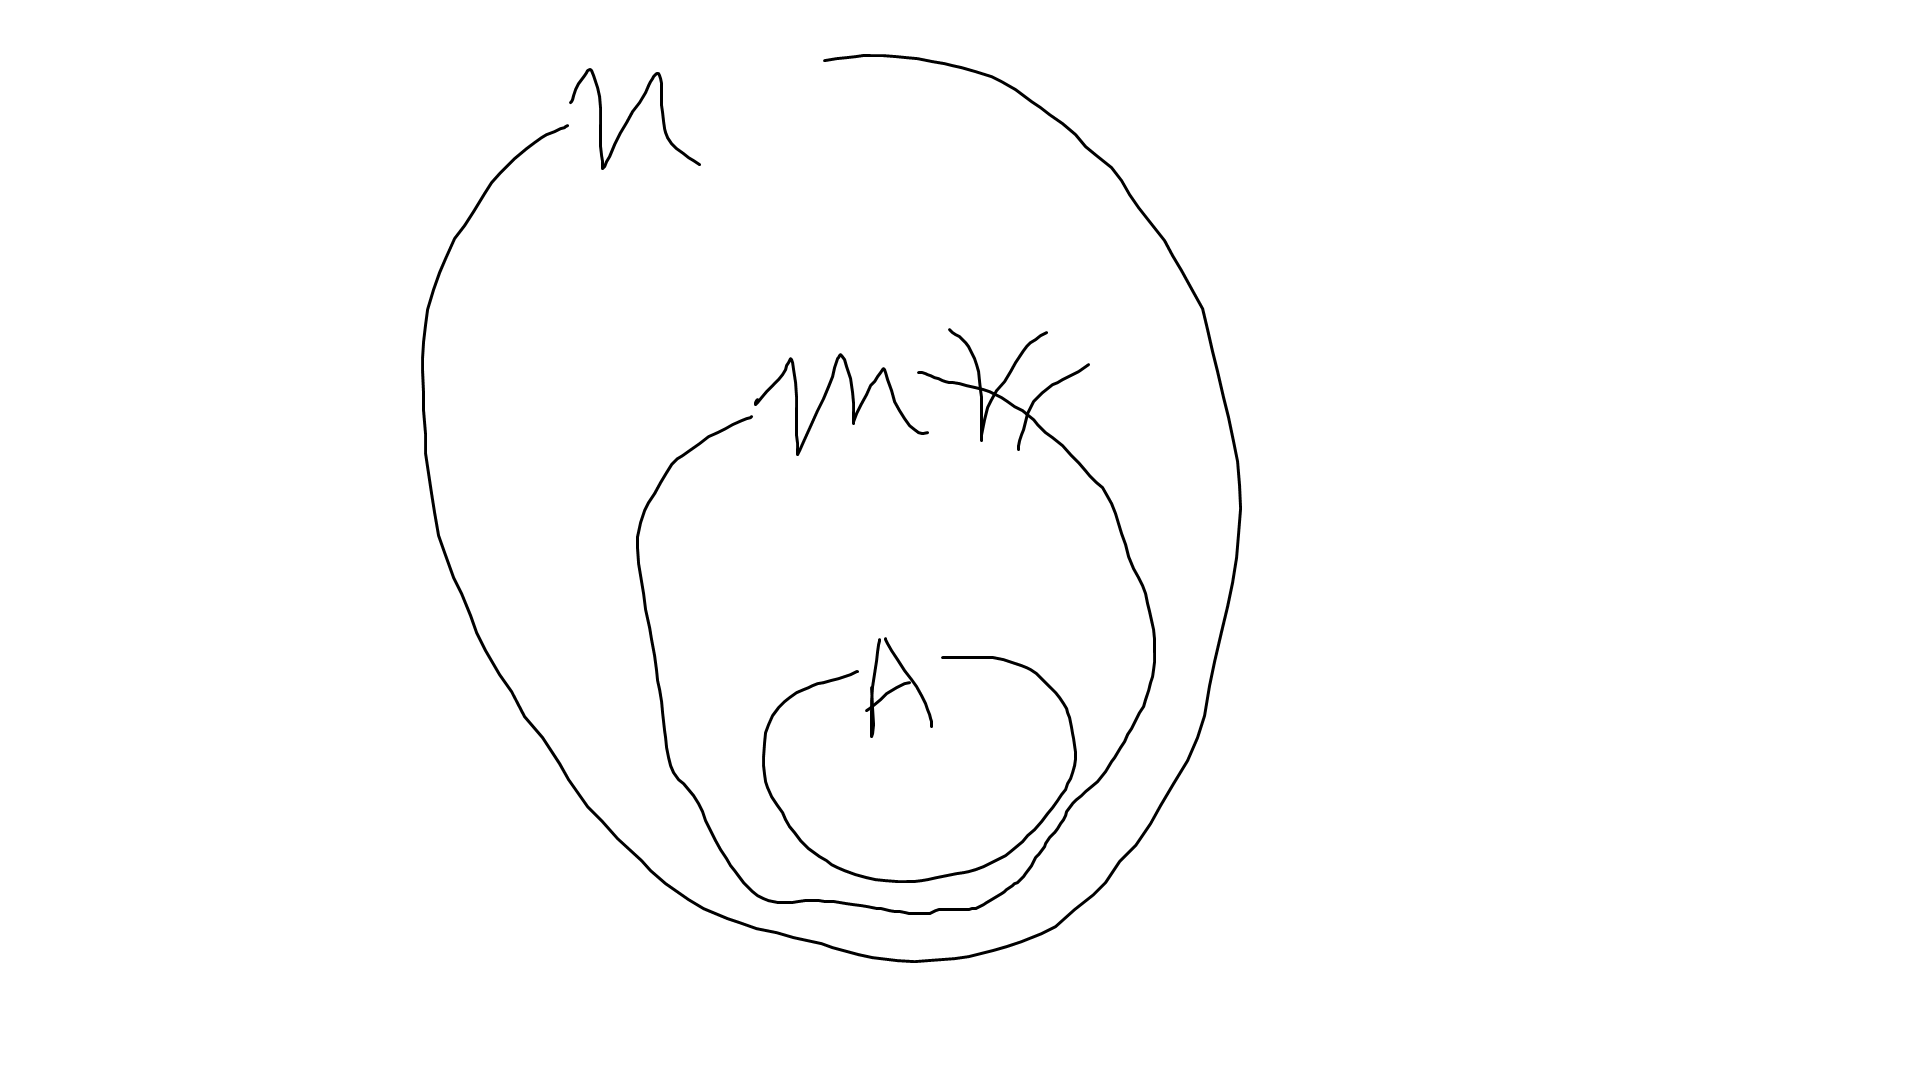
\includegraphics[scale=0.5]{image/Model_01.png}

    (It helps to think about the case $|A| = \omega$ and $|N|$ is uncountable.)\\
    A quick example how this could be useful (we'll go very sloppy here): think of $(\C,+,\cdot,-,\cdot^{-1},0,1)$ as a field. Consider $\Q \subseteq \C$ (both as subset and substructure). Note that algebraic closeness is a property of $\C$. By downward L$\ddot{o}$wenheim-Skolem, there is a substructure in $\C$ that contains $\Q$ that is als algebraically closed (apparently, the set of algebraic numbers).
    \begin{proof}
        We build a chain $\bra A_i : i < \lambda \ket$, with $A_i \subseteq N$, s.t. $|A_i| = \lambda$.\\
        (our goal: define an elementary substructure with domain $M=\bigcup_{i < \omega} A_i$).\\
        Base case: Let $A_0 \subseteq N$ be such that $A \subseteq A_0$ and $|A_0| = \lambda$.\\
        Successors: At stage $i+1$, assume $A_i$ has been built, with $|A_i| = \lambda$.\\
        Let $\bra \phi_k(x): k < \lambda \ket$ be an enumeration of those $L(A_i)$-formulas such that $\mathcal{N} \vDash \exists x \phi_k(x)$. Let $a_k$ be such that $\mathcal{N} \vDash \phi_k(a_k)$, and let $A_{i+1} = A_i \cup \{a_k: k < \lambda\}$ (basically, with those witnesses added). Then $|A_{i+1}| = \lambda$ (note that we haven't increased the size).\\
        Now let $M = \bigcup_{i < \omega} A_i$ (note the subscript range). We use lemma (3.8) to show that $M$ is the domain of $\mathcal{M} \preccurlyeq \mathcal{N}$, and $|M| = \lambda$.
        We're running out of time, so we'll continue next Monday.\\
        
        ---Lecture 5---\\
        Solutions to worksheet 1: either take along to lecture on Friday, or email them to $silvia.barbina@open.ac.uk$.

        Let's continue with the proof:

        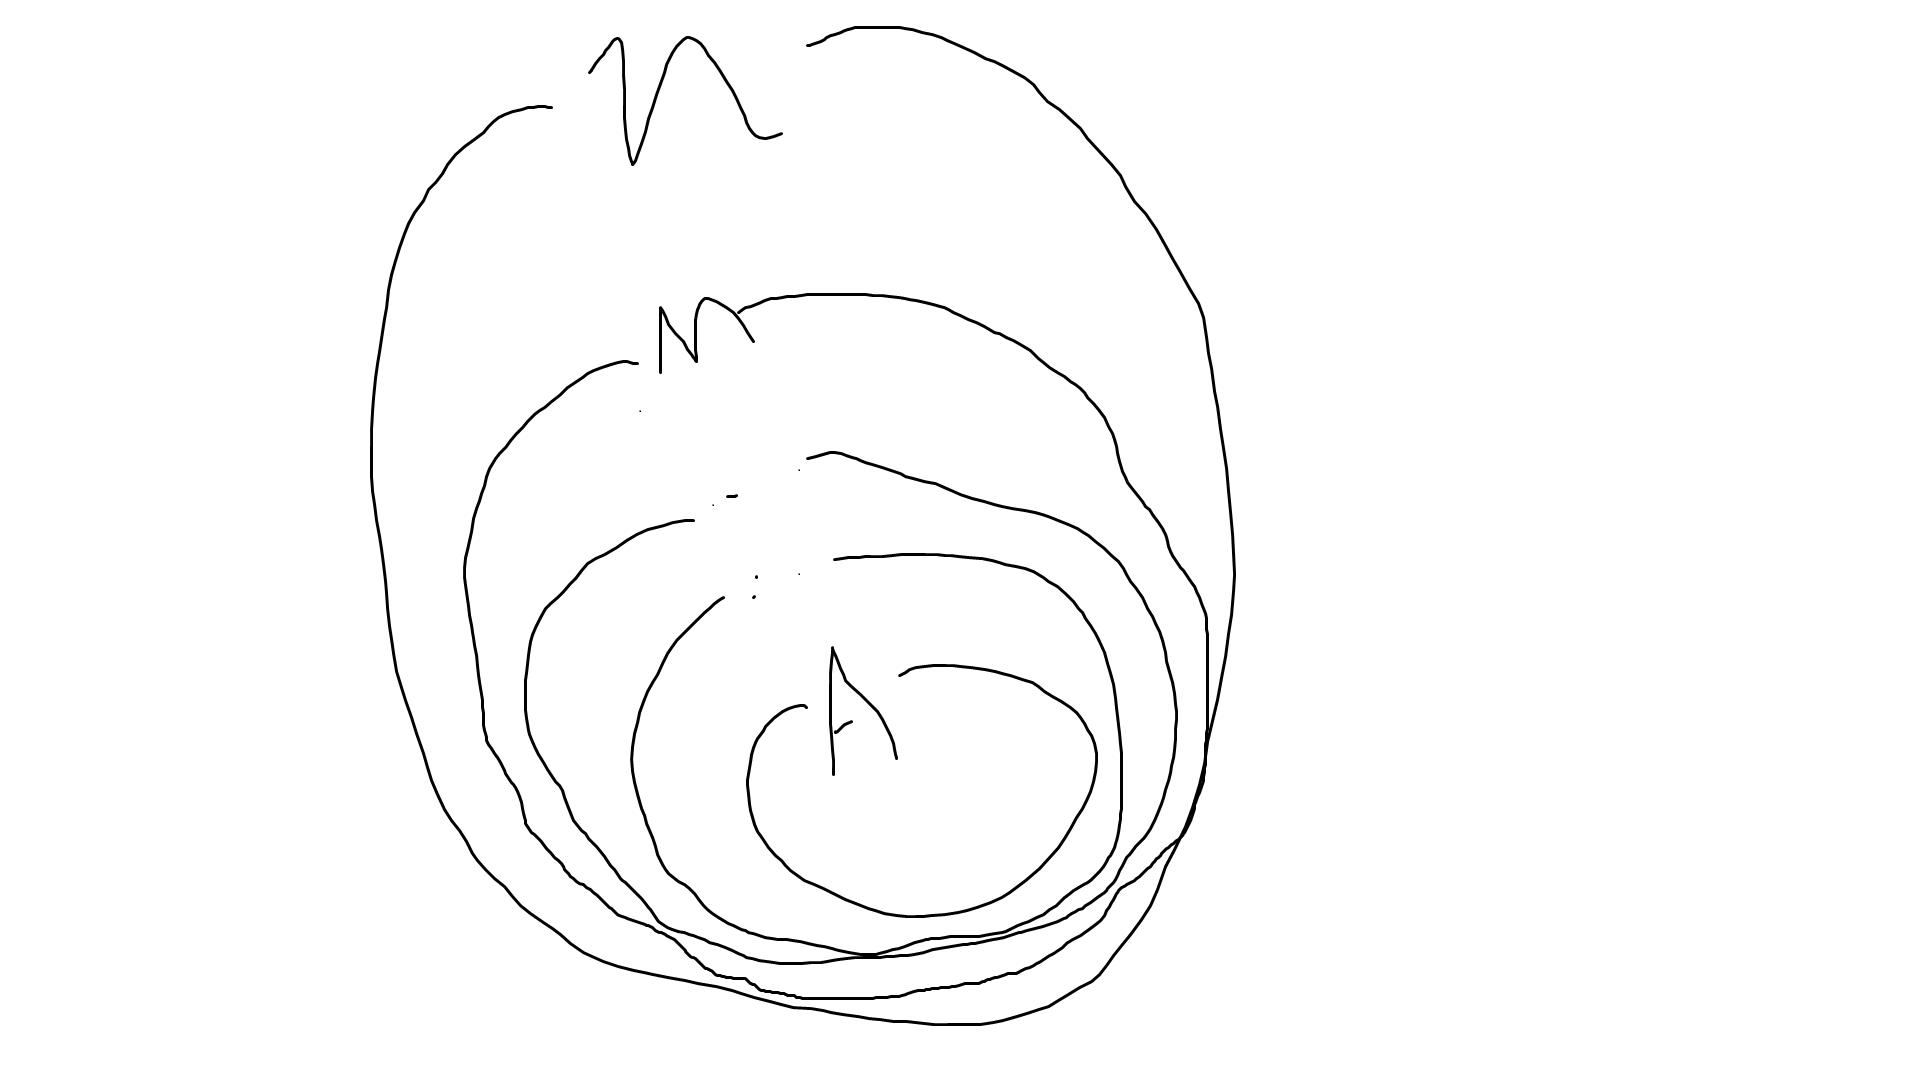
\includegraphics[scale=0.5]{image/Model_02.png}

        Start with $A_0 \subset N$, $A \subseteq A_0$, $|A_0| = l$. The idea is to define $\bra A_i: i <\omega \ket$ so that $M = \cup_{i < \omega}A_i$ satisfies (ii) via the TV test (3.8).\\
        List all formulas $\phi(x,\bar{a})$ ($\bar{a}$ is a tuple in $A_0$), and $\mathcal{N} \vDash \phi(b,\bar{a})$ for some $b$.\\
        Add each such $b$ to $A_0$ (one for each such $\phi$).\\
        Let $A_1 =A_0 \cup \{$ all thes $b$'s$\}$.\\
        Repeat for formulas $\phi(x,\bar{a})$ where $\bar{a}$ is in $A_1$,...\\
        Eventually, $\bra A_i: i<\omega\ket$ is such that $M = \cup_{i < \omega} A_i$ is as required (i.e. $M$ is the domain of some elementary substrucutre of $\mathcal{N}$ that we need).\\
        We claim that $M$ satisfies condition (ii) in Lemma (3.8): Let $\mathcal{N} \vDash \exists x \psi(x,\bar{a})$, where $\bar{a}$ is a tuple in $M$. Then $\bar{a}$ is a \emph{finite} tuple, so there is an $i$ s.t. $\bar{a}$ is in $A_i$.\\
        Then $A_{i+1}$, by construction, contains $b$ s.t. $\mathcal{N} \vDash \phi(b,\bar{a})$. But $A_{i+1} \subseteq M, b \in M$.\\
        Then apply (3.8) we're done.
    \end{proof}
\end{thm}

\newpage

\section{Two relational structures}

\begin{defi} (4.1, dense linear orders)\\
    A \emph{linear order} is an $L_{lo} = \{<\}$-structure such that:\\
    (i) $\forall x \neg (x<x)$;\\
    (ii) $\forall xyz ((x<y \wedge y<z) \to x<z)$;\\
    (iii) $\forall xy((x<y) \vee (y<x) \vee x=y)$ (total).\\
    A linear order is \emph{dense} if, in addition, it also satisfies:\\
    (iv) $\exists xy (x<y)$;\\
    (v) $\forall xy, (x<y \to \exists z (x<z \wedge z<y))$ (density).\\
    A linear order has no endpoints if, in addition, \\
    (vi) $\forall x (\exists y(x<y) \wedge \exists z(z<x))$.\\
    We use $T_{dlo}$ to denote the theory that includes all axioms (i) to (vi), and $T_{lo}$ is the theory that includes axioms (i) to (iii) only.
\end{defi}

\begin{rem}
    (iv) and (v) imply that if $\mathcal{M} \vDash T_{dlo}$, then $|\mathcal{M}| \geq \omega$.
\end{rem}

\begin{defi} (4.2)\\
    If $\mathcal{M},\mathcal{N} \vDash T_{lo}$, then an \emph{injective} map $p:A \subseteq M \to N$ is a \emph{partial embedding} if $\mathcal{M} \vDash a<b \implies \mathcal{N} \vDash p(a) < p(b)$.\\
    In particular, if $|\dom(p)| < \omega$, then $p$ is a \emph{finite} partial embedding.
\end{defi}

\begin{lemma} (4.3, extension lemma)\\
    Take a linear order $\mathcal{M} \vDash T_{lo}$, and a dense linear endpoints $\mathcal{N} \vDash T_{dlo}$, and let $p: M \to N$ be a finite partial embedding. Then if $c \in \mathcal{M}$, there is a finite partial embedding $\hat{p}$ s.t. $p \subseteq \hat{p}$ and $c \in \dom(\hat{p})$.\\
    (\emph{we can always add one extra element in our embedding}.)
    \begin{proof}
        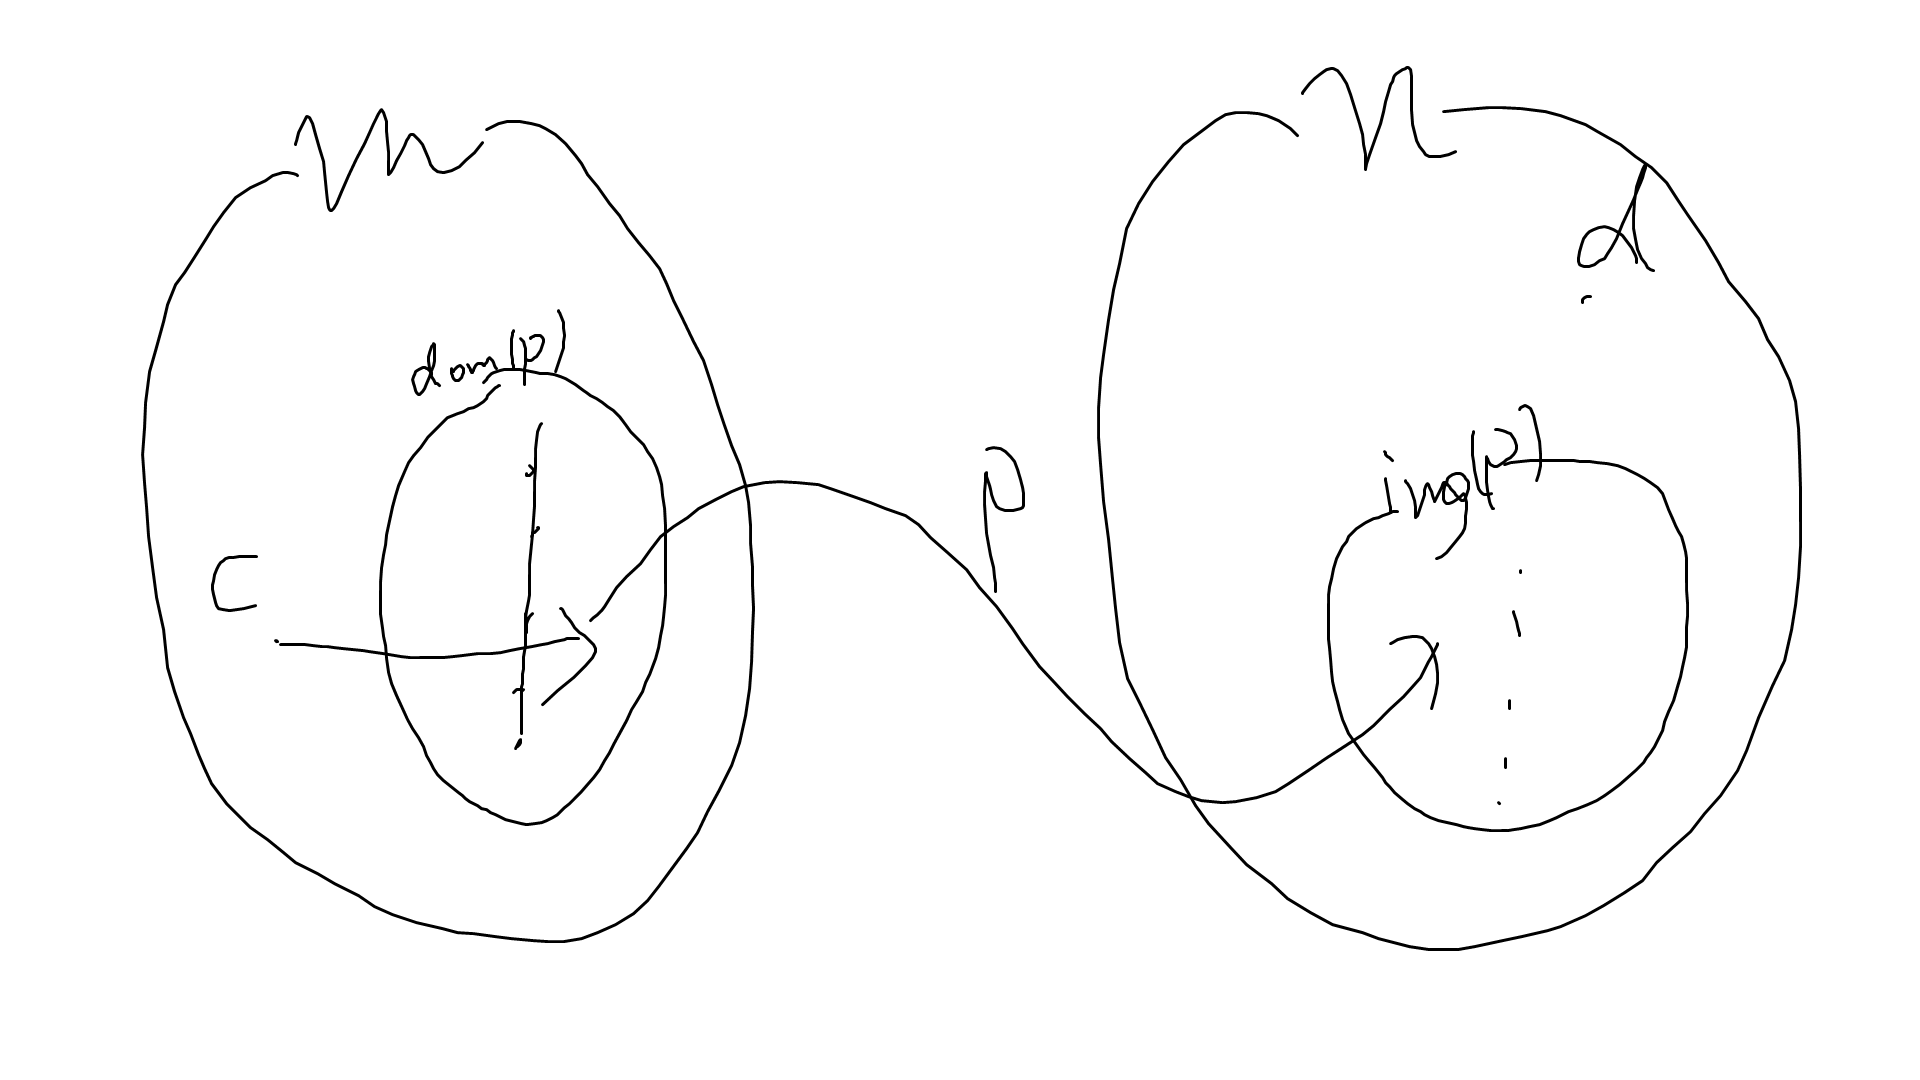
\includegraphics[scale=0.5]{image/Model_03.png}

        Case 1: $c$ is greater than all elements in $\dom(p)$. In that case, pick an element $d \in \mathcal{N}$ s.t. $d>b$ for all $b \in img(p)$;\\
        Case 2: $a_i<c<a_{i+1}$ where $a_i,a_{i+1} \in \dom(p)$. Then we choose $\mathcal{N} \vDash p(a_i) < d < p(a_{i+1})$, where $d$ is chosen appropriately by density (here's the case why we need $\mathcal{N}$ to be dense;\\
        Case 3: $c$ is less than all elements in $\dom(p)$. This is similar to case 1.

        Note that the ability to extend by one point allows us to embed any finite linear order into a dense linear order without endpoints.
    \end{proof}
\end{lemma}

\begin{thm} (4.4)\\
    Let $\mathcal{M},\mathcal{N} \vDash T_{dlo}$ s.t. $|\mathcal{M}| = |\mathcal{N}| = \omega$. Let $p:A \subseteq M \to N$ be a finite partial embedding.\\
    Then there is an isomorphism $\pi:\mathcal{M} \to \mathcal{N}$ s.t. $p \subseteq \pi$.
    \begin{proof}
        Enumerate $M,N$, say $M=\bra a_i:i < \omega\ket$, $N=\bra b_i:i < \omega\ket$ (sequences of elements).\\
        We define, inductively, a chain of finite partial embedding $\bra p_i:i<\omega\ket$ (idea: $\pi = \cup_{i<\omega} p_i$).\\
        Let's start with $p_0 = p$. At stage $i+1$, suppose we are given $p_i$. We want to include $a_i$ in $\dom p_{i+1}$, and $b_i$ in the $img(p_{i+1})$.\\
        (Lecturer calls this a \emph{back and forth} method) Forth step: By lemma 4.3, we can extend $p_i$ to $p_{i+\frac{1}{2}}$ such that $a_i \in \dom(p_{i+\frac{1}{2}})$;\\
        Back step: By lemma 4.3 again applied to $(p_{i+\frac{1}{2}})^{-1}$ to include $b_i \in \dom (p_{i+1}^{-1})$ (i.e. in the range of $p_{i+1}$).\\
        We claim that $p_{i+1}$ extends $p_i$ as required.\\
        Let $\pi = \cup_{i < \omega} p_i$. Then (check) $\pi$ is an isomorphism (i.e. order-preserving bijection).
    \end{proof}
\end{thm}

\begin{defi} (4.5)\\
    An $L$-theory is \emph{consistent} if there is $L$-structure $\mathcal{M}$ s.t. $\mathcal{M} \vDash T$.\\
    If $T$ is a theory in $L$ and $\phi$ is an $L$-sentence, then $T \vdash \phi$ (read as \emph{$T$ entails $\phi$}, note that this has nothing to do with syntactic implication) if for all $\mathcal{M}$ such that $\mathcal{M} \vDash T$, we have $\mathcal{M} \vDash \phi$; basically, $\phi$ holds in any model of $T$.\\
    Finally, an $L$-theory $T$ is \emph{complete} if for all $L$-sentences $\phi$, either $T \vdash \phi$ or $T \vdash \neg\phi$ (see part II Logic and Set Theory); so no $L$-sentence is true in only some models of $T$ but false in the others.\\
    For example, $T_{dlo}$ is complete.
\end{defi}

---Lecture 6---

\begin{defi} (4.6)\\
    A theory $T$ in a countable language with a (infinitely) countable model is \emph{$\omega$-categorical} if any two countable models of $T$ are isomorphic.
\end{defi}

\begin{coro} (4.7 of theorem (4.4))\\
    $T_{dlo}$ is $\omega$-categorical.
    \begin{proof}
        If $\mathcal{M}, \mathcal{N} \vDash T_{dlo}$, $|\mathcal{M}| = |\mathcal{N}| = \omega$, then $\phi$ (the empty map) is a finite partial embedding. But by theorem (4.4) we get $\mathcal{M} \simeq \mathcal{N}$.\\
        (We can also use any $\{\bra a,b\ket\}$ where $a \in \mathcal{M}$ and $b \in \mathcal{M}$ as initial finite partial embedding).
    \end{proof}
\end{coro}

\begin{thm} (4.8)\\
    (erratum 26th Oct 2018: lecturer wants to add a condition \emph{$T$ has no finite models}. Then the problem with (4.11) is fixed.)\\
    If $T$ is an $\omega$-categorical theory in a countable language, then $T$ is complete.
    \begin{proof}
        Let $\mathcal{M} \vDash T$ and $\phi$ be an $L$-sentence.\\
        If $\mathcal{M} \vDash \phi$, suppose $\mathcal{N} \vDash T$. Then by theorem (3.11) (Downward Lowenheim-Skolem), there are $\mathcal{M}' \preccurlyeq \mathcal{M}$, $\mathcal{N}' \preccurlyeq\mathcal{N}$ s.t. $|\mathcal{M}'| = |\mathcal{N}'| = \omega$.\\
        But $\mathcal{M}' \simeq \mathcal{N}'$ (by $\omega$-categoricity), so in particular $\mathcal{M}' \equiv \mathcal{N}'$, and so $\mathcal{N}' \vDash \phi$. By elementarity, $\mathcal{N} \vDash \phi$.\\
        The case $\mathcal{M} \vDash \neg\phi$ is similar.\\
        (Think about if $T$ could have a finite model.)
    \end{proof}
\end{thm}

\begin{coro} (4.9)\\
    $T_{dlo}$ is complete.
\end{coro}

\begin{defi} (4.10)\\
    If $\mathcal{M}$, $\mathcal{N}$ are $L$-structures, a map $f$ such that $\dom (f) \subseteq M$ (the domain of $\mathcal{M}$), and $img(f) \subseteq N$ is a (partial) \emph{elementary map} if for all $L$-formulas $\phi(\bar{x})$ and $\bar{a} \in (\dom(f))^{|\bar{x}|}$, then
    $$\mathcal{M} \vDash \phi(\bar{a}) \iff \mathcal{N} \vDash \phi(f(\bar{a}))$$
\end{defi}

\begin{rem} (4.11)\\
    A map $f$ is elementary iff every finite restriction of $f$ is elementary.\\
    (Why? For forward, if $f_0 \subseteq f$ is a finite restriction that is not elementary, then for some formula $\phi(\bar{x})$, $\bar{a} \in \dom (f_0)$, the above equivalence doesn't hold; but then that equivalence doesn't hold for $f$ either; contradiction; for backward, if $f$ is not elementary, then the above equivalence fails on a finite tuple, so the above equivalence fails on some finite restriction.)
\end{rem}

\begin{prop} (4.12)\\
    Let $\mathcal{M},\mathcal{N} \vDash T_{dlo}$, and let $p: A \subseteq M \to N$ be a partial embedding. Then $p$ is elementary.\\
    \begin{proof}
        By remark (4.11), it suffices to consider $p$ finite.\\
        By Downward L-S theoem (3.11), we choose $\mathcal{M}',\mathcal{N}'$ such that\\
        (i) $|\mathcal{M}'| = |\mathcal{N}'| = \omega$;\\
        (ii) $\mathcal{M}' \preccurlyeq\mathcal{M}$, $\mathcal{N}' \preccurlyeq\mathcal{N}$;\\
        (iii) $\dom (p) \subseteq M', img(p) \subseteq N'$.

        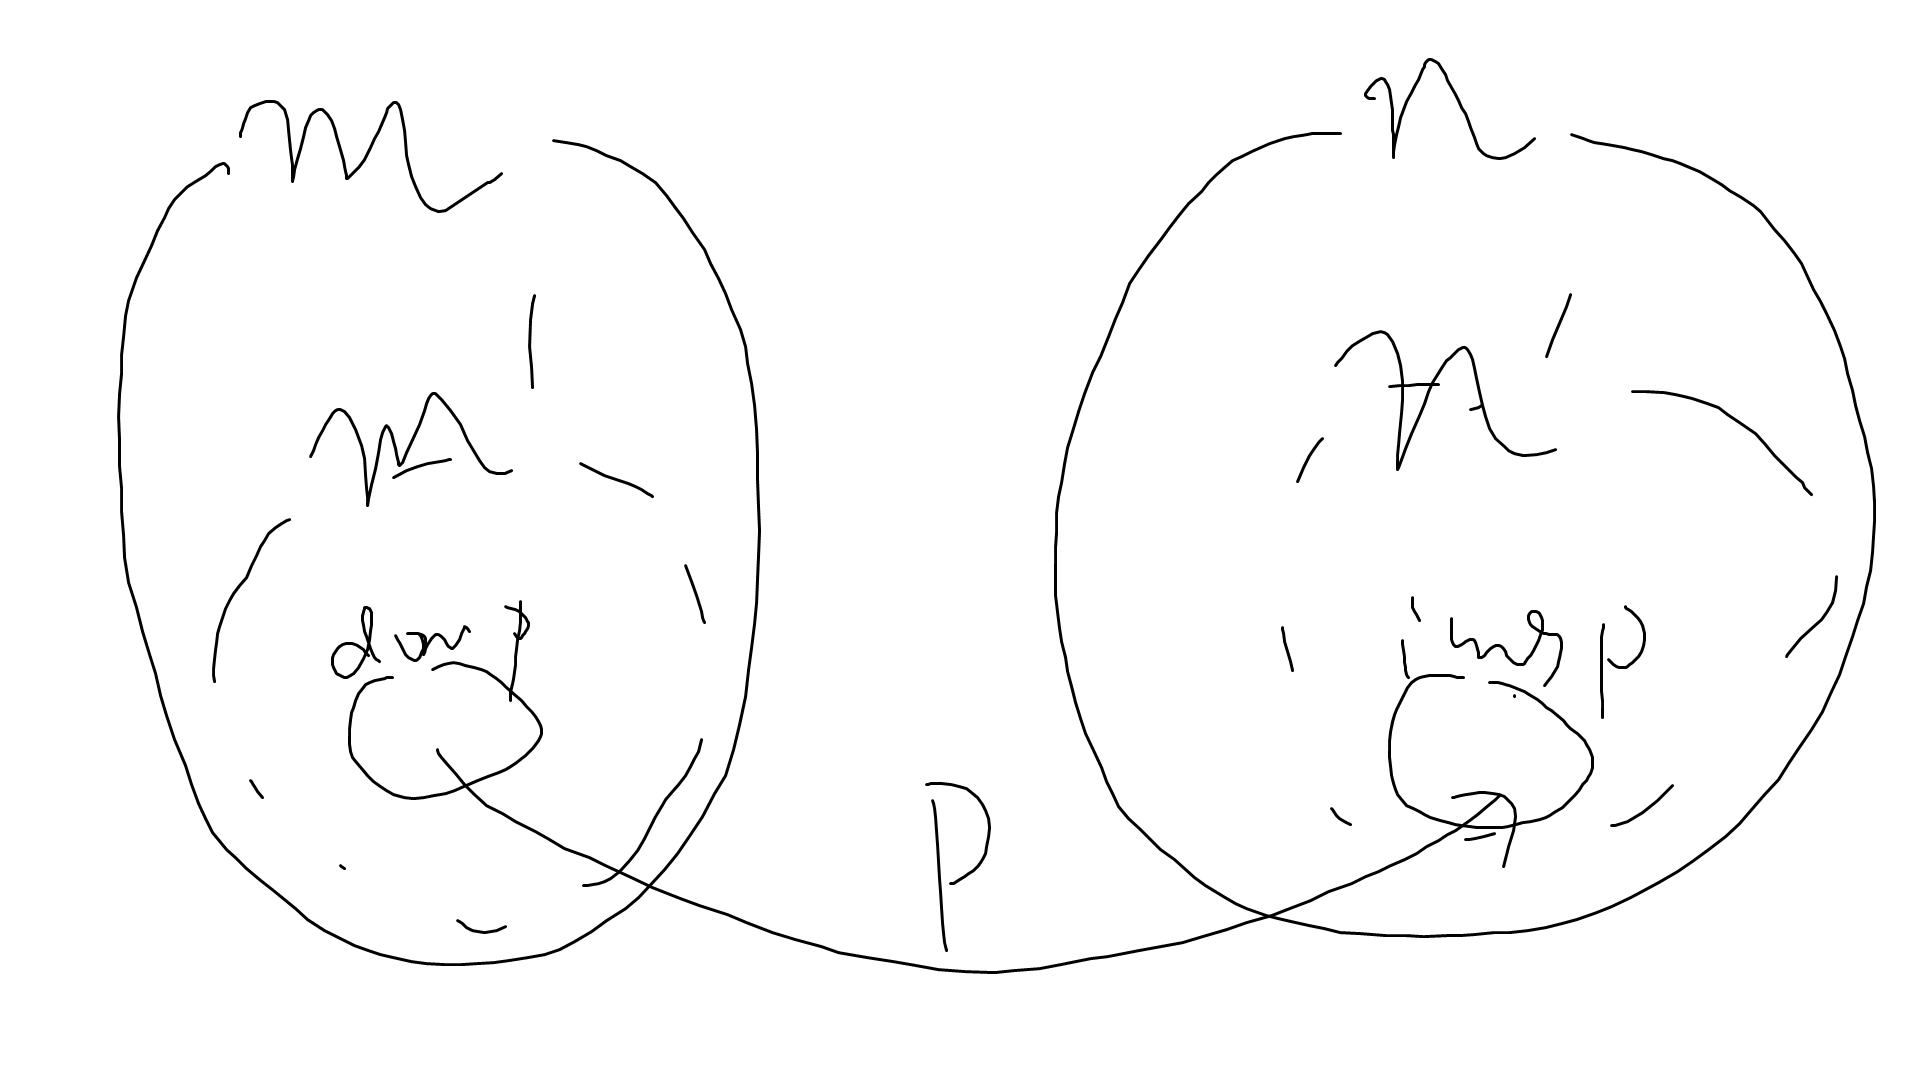
\includegraphics[scale=0.5]{image/Model_04.png}

        Now $p$ is a finite partial embedding between countable models, so $p$ extends to an isomorphism $\pi:\mathcal{M}' \to \mathcal{N}'$.\\
        In particular, $\pi$ is an elemntary map between $\mathcal{M}$ and $\mathcal{N}$.
    \end{proof}
\end{prop}

\begin{coro} (4.13)\\
    $(\Q,<) \preccurlyeq (\R,<)$.\\
    \begin{proof}
        Use proposition (4.12) with $id:\Q \to \R$.
    \end{proof}
\end{coro}

\begin{defi} (4.14)\\
    (See Part II Logic and Set Theory)\\
    Let $L_{gph} = \{R\}$, where $R$ is a binary relation symbol.\\
    An $L_{gph}$-structure is a graph if\\
    (i) $\forall x$ $\neg R(x,x)$;\\
    (ii) $\forall xy (R(x,y) \leftrightarrow R(y,x))$.

    An $L_{gph}$-structure is a \href{http://modeltheory.wikia.com/wiki/Random_graph}{random graph} if it is a graph such that the following axiom-schema $(r_n)$ hold:

    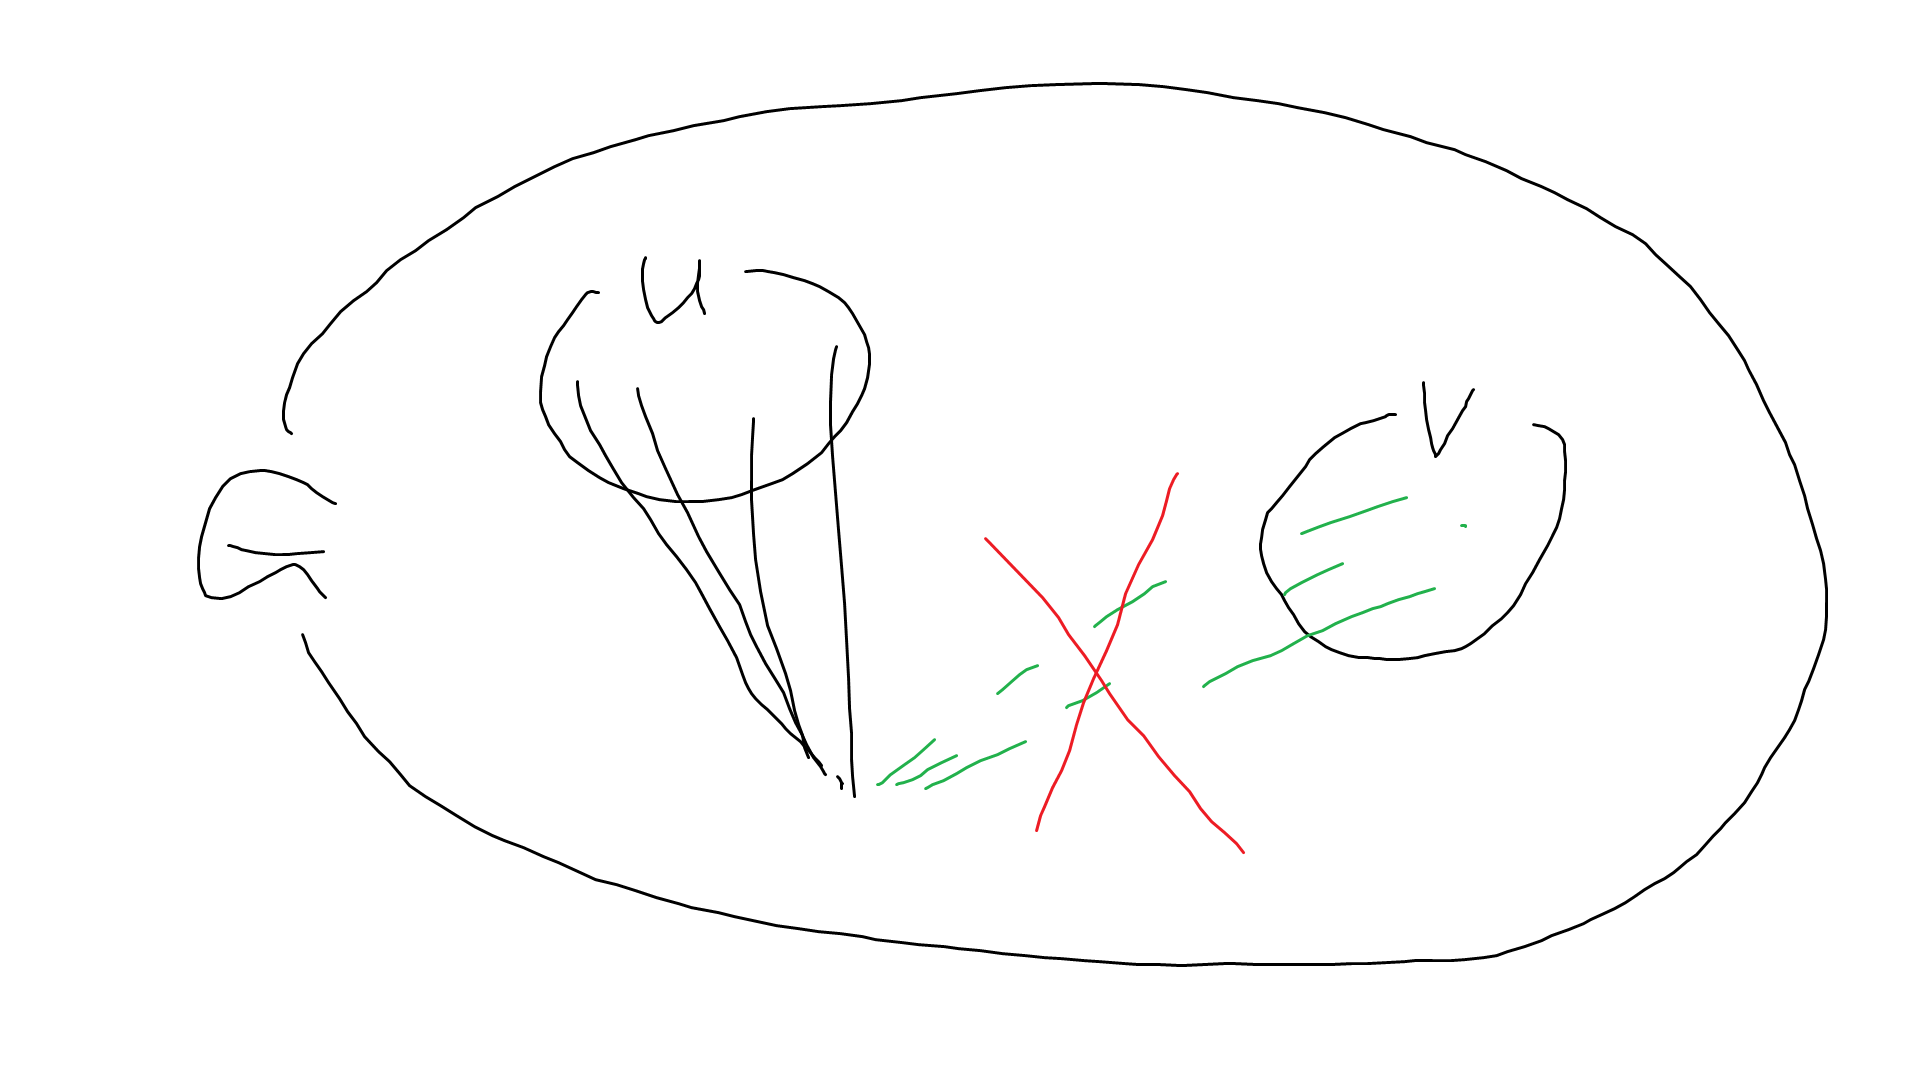
\includegraphics[scale=0.5]{image/Model_05.png}

    $$\forall x_0...x_n,y_0...y_n, (\bigwedge_{i,j=0}^n x_i \neq y_j \to \exists z(\bigwedge_{i = 0}^n (z \neq x_i) \wedge (z \neq y_i) \wedge R(z,x_i) \wedge \neg R(z,y_i)))$$

    (iii) $\exists xy (x\neq y)$.
\end{defi}

\begin{rem} (similar to what is mentioned in the link above)\\
    A random graph is infinite. Given a finite subset, we can always find a vertex that is connected to every vertex in the subset (likewise for not connected).
\end{rem}

\begin{fact} (4.15)\\
    There is a random graph.
    \begin{proof}
        Let the domain be $\omega$, let $i,j \in \omega$ such that $i < j$. Write $j$ as a sum of distinct powers of $2$. Then $\{i,j\}$ is an edge iff $2^i$ appears in the sum.\\
        As an exercise, prove that $\omega$ with this definition of $R$ is indeed a random graph.
    \end{proof}
\end{fact}

\begin{defi} (4.16, or more precisely just notations)\\
    $T_{gph} = \{$axioms (i), (ii)$\}$, $T_{rg} = T_{gph} \cup \{$(iii), ($r_n$) $:n \in \omega\}$.\\
    If $\mathcal{M},\mathcal{N} \vDash T_{gph}$, a partial embedding is an injection $p: A \subseteq M \to N$ s.t. $\mathcal{M} \vDash R(p(a),p(b)) \iff \mathcal{N} \vDash R(a,b)$ for all $a,b$ in the domain.
\end{defi}

\begin{lemma} (4.17)\\
    Let $\mathcal{M} \vDash T_{gph},\mathcal{N} \vDash T_{rg}$, let $p:A \subseteq M \to N$ be a finite partial embedding, and let $c \in M$.\\
    Then there is a map $\hat{p}:\hat{A} \subseteq M \to N$ such that $\hat{p}$ is a partial embedding, $c \in \dom \hat{p}$, $p\subseteq \hat{p}$.\\
    (This is like another extension lemma.)\\
    We'll prove this next time.
    
    ---Lecture 7---

    Last time we defined what a random graph is (in this course). We also defined what is a partial embedding in this theory (just preserves all edges).\\
    Let's continue with the proof of the lemma now. Let $c \in M$, $c \not\in \dom(p)$.

    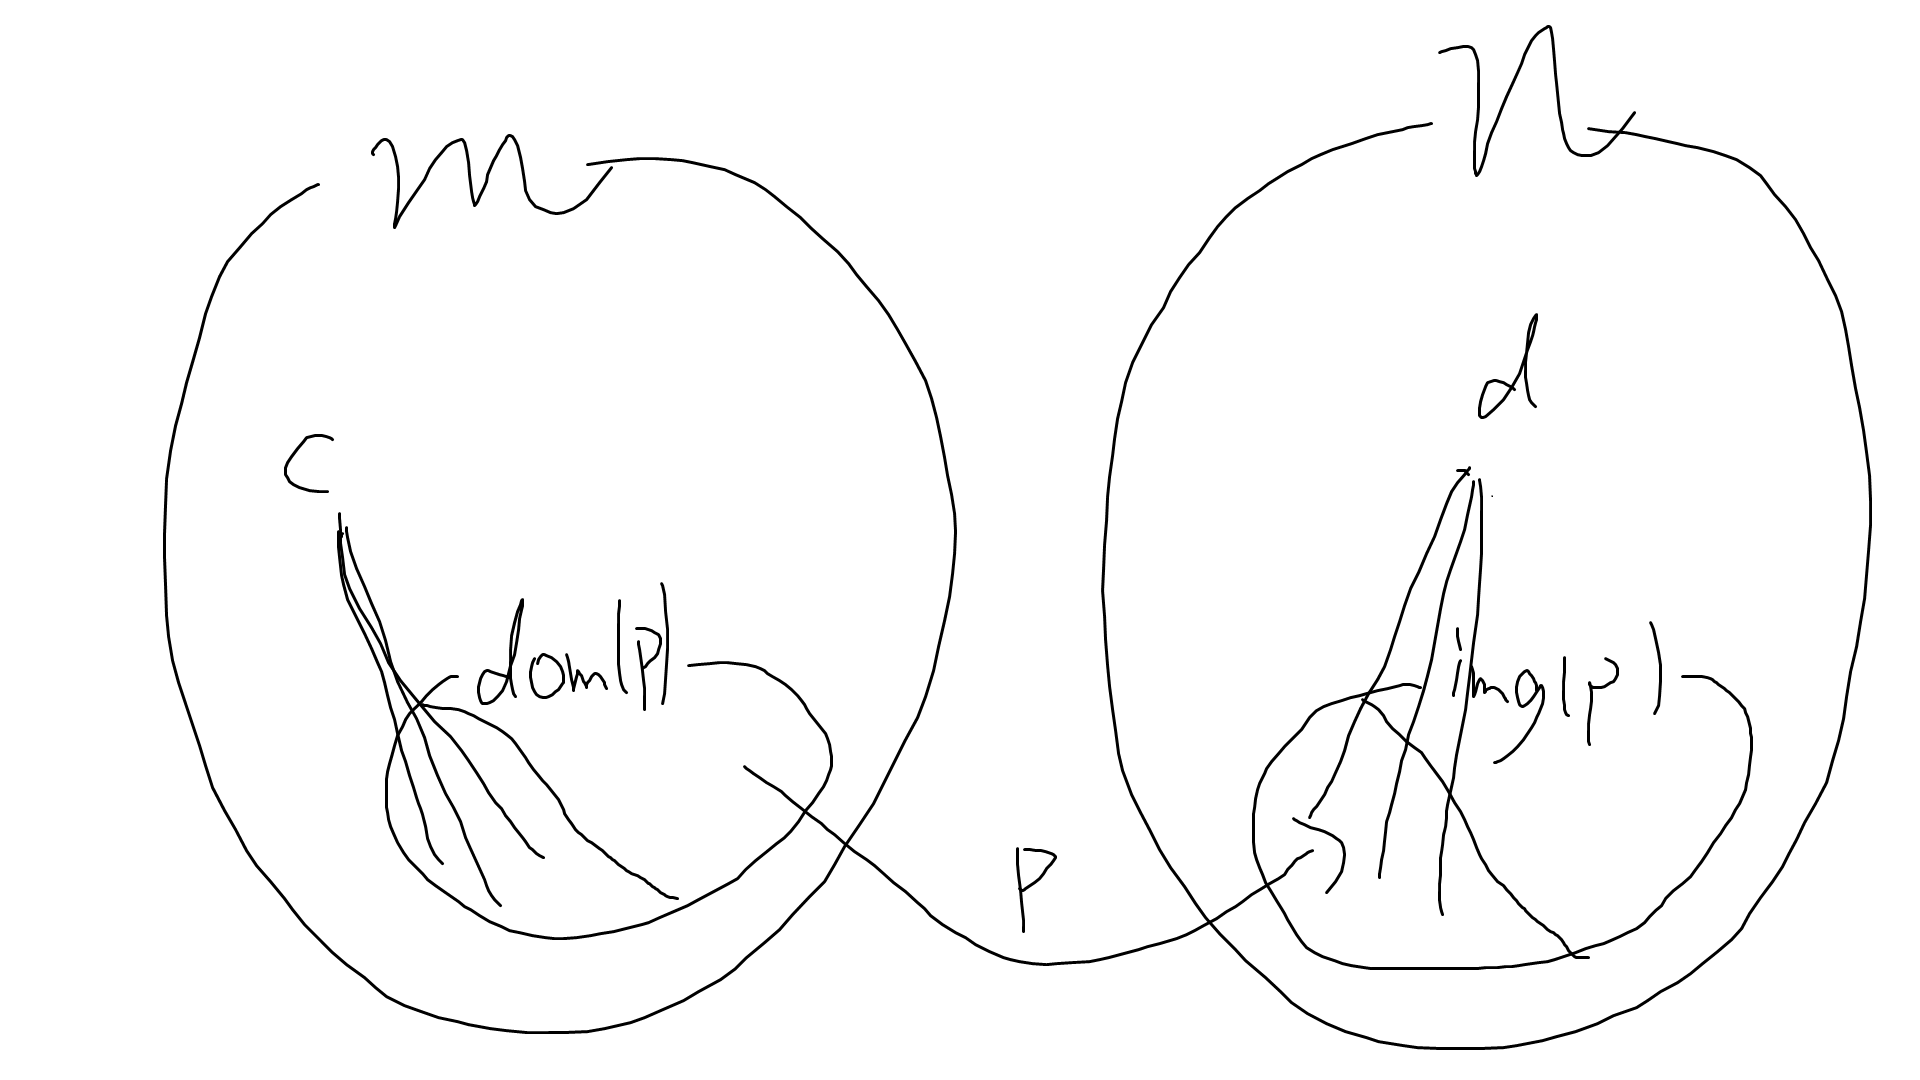
\includegraphics[scale=0.5]{image/Model_06.png}

    Find $d \in N$ such that $\mathcal{N} \vDash R(d,p(a)) \iff \mathcal{M} \vDash R(c,a)$.
\end{lemma}

\begin{thm} (4.18)\\
    Let $\mathcal{M},\mathcal{N} \vDash T_{rg}$ and $|\mathcal{M}| = |\mathcal{N}| = \omega$, and $P:A \subseteq M \to N$ is a finite partial embedding.\\
    Then $\mathcal{M} \simeq \mathcal{N}$, by an isomorphism that extends $p$.
    \begin{proof}
        Same as proof of Theorem (4.4) (there is only one model of $T_{dlo}$ up to isomorphism), but with lemma (4.17) instead of lemma (4.3).
    \end{proof}
\end{thm}

\begin{coro} (4.19)\\
    $T_{rg}$ is $\omega$-categorical (see definition (4.6) -- this is just a restatement of the theorem above) and complete.\\
    In particular, every finite partial embedding between models of $T_{rg}$ is an elementary map.
\end{coro}

\begin{rem}
    The unique (up to isomorphism) model of $T_{rg}$ is \emph{the} countable random graph, or the \emph{Rado} graph.\\
    It is universal w.r.t. finite and countable graphs (i.e. it embeds all).\\
    Another nice property (which you are not required to see this immediately -- it is far from trivial) \emph{ultrahomogeneous}, i.e. every isomorphism between finite substructures extends to an automorphism of the whole graph.\\
    Google \emph{David Marker's} book, or \emph{Tent-Ziegler}. Warning: both of them contain a lot of typos.
\end{rem}

\newpage

\section{Compactness}

\begin{defi} (5.1)\\
    Suppose we have a $L$-theory $T$.\\
    (i) $T$ is \emph{finitely satisfiable} if every finite subset of sentences in $T$ has a model.\\
    (ii) $T$ is \emph{maximal} if for all $L$-sentences $\sigma$, either $\sigma \in T$ or $\neg\sigma \in T$.\\
    (iii) $T$ has the \emph{witness property} (WP): if for all $\phi(x)$ ($L$-formula with $1$ free variable), there is a constant $c \in \mathcal{C}$ s.t.
    $$(\exists x \phi(x) \to \phi(c)) \in T$$
\end{defi}

\begin{lemma} (5.2)\\
    If $T$ is maximal and finitely satisfiable (we'll sometimes use \emph{f.s.} from now onwards), and $\phi$ is an $L$-sentence, and $\triangle \stackrel{fin}{\subseteq} T$ and $\triangle \vdash \phi$, then $\phi \in T$.\\
    (Prove it by yourself)
\end{lemma}

\begin{lemma} (5.3)\\
    Let $T$ be a maximal, f.s. theory with WP. Then $T$ has a model.\\
    Moreover, if $\lambda$ is a cardinal and $|\mathcal{C}| \leq \lambda$ ($\mathcal{C}$ is the set of constants in $L$), then $T$ has a model of size at most $\lambda$.
    \begin{proof}
        Let $\mathcal{C}$ be the constants of $L$. Let $c,d \in \mathcal{C}$, define $c \sim d$ iff $c=d \in T$.\\
        We claim that $\sim$ is an equivalence relation: reflexivity and symmetry are trivial; for transitivity, let $c \sim d$ and $d \sim e$. Then $c=d \in T$ and $d=e \in T$. Then by the lemma $c=e\in T$ as it is implied by the two sentences. So $c \sim e$.\\
        Notation: we'll use $c/\sim = c^*$ to denote the equivalence class of $c$.\\
        Now define a structure $\mathcal{M}$ whose domain is $\mathcal{C}/\sim = M$. Clearly, $|M| \leq \lambda$ if $|\mathcal{C}| \leq \lambda$.\\
        We must define interpretations in $\mathcal{M}$ for symbols for $L$:\\
        $\bullet$ If $c \in \mathcal{C}$, then $c^m = c^* (=c/\sim$);\\
        $\bullet$ If $R \in \mathcal{R}$ is a relation symbol, we define $R^{\mathcal{M}} = \{(c_1^*,...,c_{n_R}^*):R(c_1,...,c_{n_R}) \in T\}$.\\
        We have to check that $R^{\mathcal{M}}$ is well-defined: suppose $\bar{c},\bar{d} \in \mathcal{C}^{n_R}$ and suppose $c_i \sim d_i$ for each $i$, i.e. $c_i = d_i \in T$ for every $i=1,...,n_R$. However, now
        $$R(\bar{c}) \in T \iff R(\bar{d}) \in T$$
        by maximality of $T$ and the previous lemma. So that $R^{\mathcal{M}}$ is well defined.\\
        $\bullet$ If $f \in \mathcal{F}$ is a function symbol, then $f(\bar{c}) = d \in T$ for some $d \in \mathcal{C}$: this is because $\exists x(f(\bar{c})=x) \in T$ by maximality and f.s..\\
        Then define $f^{\mathcal{M}}(\bar{c}^*) = \bar{d}^*$ (obvious notation).\\
        We also have to check this is well-defined. Lecturer decides to left this to us.\\
        Now we claim that the terms behave nicely as what the theory says, i.e. if $t(x_1,...,x_n)$ is an $L$-term and $c_1,...,c_n,d \in \mathcal{C}$, then $t(c_1,...,c_n) = d \in T \iff t^{\mathcal{M}} (c_1^*,...,c_n^*) = d^*$.\\
        $\bullet$ $\implies$: by induction on the complexity of $T$ (lecturer decided to leave this as another exercise).\\
        $\bullet$ $\Leftarrow$: Assume $t^{\mathcal{M}} (c_1^*,...,c_n^*) = d^*$. Then $t(c_1,...,c_n) = e \in T$ for some constant $e$ (why? As our theory is maximal, it has to say what the result is when we apply $t$ to these terms). We then use $\implies$ to get that $t^{\mathcal{M}}(c_1^*,...,c_n^*) = e^*$.\\
        But then $d^* = e^*$, i.e. $d = e \in T$. So by lemma (5.2), the sentence implied by these two sentences, $t(c_1,...,c_n) = d \in T$.\\
        The last massive claim: for all $L$-formulas $\phi(\bar{x})$ and $\bar{c} \in \mathcal{C}^{|\bar{x}|}$, we have
        $$\mathcal{M} \vDash \phi(\bar{c}) \iff \phi(\bar{c}) \in T$$
        The proof is by induction on complexity of $\phi(\bar{x})$ (The lecturer decided to leave yet another proof to us -- lots of work to be done here. Lecturer is speeding up!).
    \end{proof}
\end{lemma}

---Lecture 8---

\begin{lemma} (5.4)\\
    Let $T$ be a f.s. $L$-theory. Then there are $L^* \supseteq L$ and a f.s. $T^* \supseteq T$ such that:\\
    (i) $|L^*| = |L| + \omega$;\\
    (ii) any $L^*$-theory extending $T^*$ has WP.
    \begin{proof}
        Define $\bra L_i: i < \omega \ket$ a chain of languages containing $L$ and s.t. $|L_i| = |L|+\omega$, and $\bra T_i: i < \omega \ket$ of f.s. theories s.t. $\forall i$ $T_i$ is an $L_i$-theory, and $T_i \supseteq T$.\\
        $\bullet$ Base step: $L_0=L$ and $T_0=T$.\\
        $\bullet$ At stage $i+1$, $L_i$ and $T_i$ are given. List all $L_i$-formulas $\phi(x)$ (one free variable $x$) and let $L_{i+1} = L_i \cup \{c_\phi:\phi(x)$ is an $L_i$-formula$\}$.\\
        For all $\phi(x)$ ($L_i$-formula), let $\Phi_\phi$ be the $L_{i+1}$-sentence $\exists x\phi(x) \to \phi(c_\phi)$.\\
        Then $T_{i+1}:= T_i \cup \{\Phi_\phi: \phi(x)$ is $L_i$-formula$\}$.\\
        Claim: $T_{i+1}$ is f.s.. Why is that? Let's take a finite subset $\triangle \stackrel{fin}{\subseteq} T_{i+1}$. Then $\triangle = \triangle_0 \cup \{\Phi_{\phi_2},...,\Phi_{\phi_n}\}$ where $\triangle_0 \subseteq T_i$.\\
        Let $\mathcal{M} \vDash \triangle_0$ ($\mathcal{M}$ is an $L_i$-structure; it exists because $T_i$ is f.s.).\\
        We define an $L_{i+1}$-structure $\mathcal{M'}$ with domain $M$ (of $\mathcal{M}$). Define the integration of new constants as follows: if $\mathcal{M} \vDash \exists x \phi(x)$, then $c_\phi^{\mathcal{M}'} = a$ for any $a \in \mathcal{M}$ s.t. $\mathcal{M} \vDash \phi(a)$.\\
        Otherwise, $c_\phi^{\mathcal{M}'}$ is arbitrary.\\
        Then $\mathcal{M}' \vDash \triangle$.\\
        Now let $L^* = \cup_{i < \omega} L_i$, $T^* = \cup_{i<\omega} T_i$.\\
        By our construction, any extension of $T^*$ has WP (check), and $T^*$ is f.s. ($\triangle \stackrel{fin}{\subseteq} T^*$, then $\triangle \subseteq T_i$ for some $i$). 
    \end{proof}
\end{lemma}

\begin{lemma} (5.5)\\
    If $T$ is f.s., there exists a maximal f.s. $T' \supseteq T$ (of underlying language $L$).
    \begin{proof}
        Let $I:= \{ S: S$ is a f.s. $L$-theory s.t. $T \subseteq S\}$.\\
        $I$ is partially ordered by inclusion.\\
        If $\bra C_i: i < \lambda\ket$ is a chain in $I$, then $\cup_{i < \lambda} C_i$ is an upper bound for the chain: it is f.s. ($\triangle \subseteq \cup C_i$ is s.t. $\triangle \subseteq C_i$).\\
        Then by Zorn's lemma, $I$ has a maximal element (w.r.t. $\subseteq$).\\
        We claim that the maximal element $T'$ of $I$ is the required extension of $T$ (check that $\forall$ $L$-sentences $\sigma$, $\sigma \in T'$ or $\neg \sigma \in T'$).
    \end{proof}
\end{lemma}

\begin{thm} (5.6, Compactness)\\
    If $T$ is a f.s. $L$-theory, and $\lambda \geq |L|+\omega$, then there is $\mathcal{M} \vDash T$ s.t. $|\mathcal{M}| \leq \lambda$.\\
    (See part II Logic and Set Theory for the finite case).\\
    \begin{proof} (sketch)\\
        Extend $T$ to $T^*$, an $L^*$-theory that is f.s., and s.t. any $S \supseteq T^*$ has WP (by lemma (5.4)).\\
        By lemma (5.5), we can extend this $T^*$ to a maximal f.s. theory $T'$; and by the lemma $T'$ would have WP since it is an extension of $T^*$.\\
        Now $T'$ is maximal and f.s., so we can use lemma (5.3) to show that there is a model $\mathcal{M} \vDash T'$. Then in particular, $\mathcal{M} \vDash T$ (check $\mathcal{M} \leq \lambda$).
    \end{proof}
\end{thm}

\begin{defi} (5.7)\\
    Let $L$ be a language. Then an $L$-type $p(\bar{x})$ is a set of $L$-formulas whose free variables are in $\bar{x}$ (and $\bar{x} = \bra x_i : i < \lambda \ket $).\\
    $\bullet$ An $L$-type is \emph{satisfiable} if there is an $L$-structure $\mathcal{M}$ and an assignment $\bar{a} \in \mathcal{M}^{|\bar{x}|}$ s.t. $\mathcal{M} \vDash \phi(\bar{a})$ for all $\phi(\bar{x}) \in p(\bar{x})$ (we also say $p(\bar{x})$ is \emph{consistent}, and $\bar{a}$ \emph{realizes} $p(\bar{x})$ in $\mathcal{M}$).\\
    We write $\mathcal{M} \vDash p(\bar{a})$, or $\mathcal{M},\bar{a} \vDash p(\bar{x})$.\\
    We also say that $p(\bar{x})$ is \emph{satisfied in $\mathcal{M}$}.\\
    $\bullet$ A type $p(\bar{x})$ is finitely satisfiable if every finite subset of $p(x)$ is satisfiable (we may say $p(x)$ is finitely consistent).
\end{defi}

\begin{rem}
    An $L$-type may be finitely satisfiable in a model $\mathcal{M}$ (by this we mean every finite subset is satisfiable in $\mathcal{M}$), but not satisfiable in $\mathcal{M}$.
\end{rem}

\begin{eg}
    Let $\mathcal{M} = (\N,<)$. Let $\phi_n(x)$ say \emph{there are at least $n$ elements less than $x$}, and $p(x):=\{\phi_n(x):n < \omega\}$.\\
    Is $p(x)$ finitely satisfiable in $\mathcal{M}$? Yes; but obviously $p(x)$ is not satisfiable in $\mathcal{M}$.
\end{eg}

\begin{thm} (5.8)\\
    Every finitely satisfiable $L$-type $p(\bar{x})$ is satisfiable (not necessarily in the original model, of course).
    \begin{proof}
        Let $\bar{x} = \bra x_i : i<\lambda\ket$, let $\bra c_i:i<\lambda\ket$ be new constants (not in $L$).\\
        Expand $L$ to $L' = L \cup \{c_i:i<\lambda\}$. Then $p(\bar{c})$ is an $L'$-theory, and theorem (5.6) applied to $p(\bar{c})$ gives the desired conclusion (think).
    \end{proof}
\end{thm}

---Lecture 9---

Example class 2: 19th November, Monday.

\begin{lemma} (5.9)\\
    Let $\mathcal{M}$ be a structure, let $\bar{a} = \bra a_i:i<\lambda \ket$ enumerate $\mathcal{M}$. Let
    $$q(\bar{x}) = \{\phi(\bar{x}): \mathcal{M} \vDash \phi(\bar{a})\}$$
    where $|\bar{x}| = \lambda$.\\
    Then $q(\bar{x})$ is satisfiable in $\mathcal{N}$ iff there is $\beta:\mathcal{M} \to \mathcal{N}$ that is an elementary embedding.
    \begin{proof}
        If $q(\bar{x})$ is satisfiable in $\mathcal{N}$, there is $\bar{b} \in N^{|\bar{x}|}$ s.t. $\mathcal{N} \vDash \phi(\bar{b})$ for all $\phi(\bar{x}) \in q(\bar{x})$.\\
        Then $\beta:a_i \to b_i$ ($i < \lambda$) is an elementary embedding ($\beta$ preserves, for example, atomic formulas of the form $f(a_{i_1},...,a_{i_n}) = a_{i_{n+1}}$, so it is an embedding.)\\
        More generally, for any $\phi(\bar{x})$ ($L$-formula),\\
        $\mathcal{M} \vDash \phi(\bar{a})$ iff $\mathcal{N} \vDash \phi(\bar{b})$, but $\beta(\bar{a}) = \bar{b}$.\\
        Conversely, if $\beta:\mathcal{M} \to \mathcal{N}$ is elementary, then $\beta(\bar{a})$ satisfies $q(\bar{x})$ in $\mathcal{N}$.
    \end{proof}
\end{lemma}

\begin{rem}
    The above is usually stated as (diagram lemma): Let $Th(\mathcal{M}_M)$ be a theory in $L(M)$, $\mathcal{N} \vDash Th(\mathcal{M}_M)$, then $\mathcal{M}$ embeds elementarily in $\mathcal{N}$.
\end{rem}

\begin{rem} (5.10)\\
    We can consider types in $L(A)$, where $A \subseteq \mathcal{M}$.\\
    In particular, we can consider $A=M$ the whole domain of $\mathcal{M}$.\\
    Types of this kind are said to \emph{have parameters in $A$} (or to be \emph{over $A$}).\\
    If $p(\bar{x})$ is a type over $M$, then there is a $\bar{a}$, an enumeration of $M$, and a type $p'(\bar{x},\bar{z})$ where the $\bar{z}$ are \emph{new constants}, $|\bar{z}| = |\bar{a}|$, and $p(\bar{x}) = p'(\bar{x},\bar{a})$.
\end{rem}

\begin{thm} (5.11)\\
    If $\mathcal{M}$ is a structure, and $p(x)$ is a type in $L(M)$ that is finitely satisfiable in $\mathcal{M}$, then $p(\bar{x})$ is satisfiable in some $\mathcal{N}$ such that $\mathcal{M} \preccurlyeq \mathcal{N}$.
\end{thm}

\begin{eg}
    Consider $\mathcal{M} = (\Q,<)$, and let $\bra a_i:i < \omega\ket$ a sequence in $\Q$ that converges to $\sqrt{2}$ from below, and let $\bra b_i:i < \omega\ket \subseteq \Q$ tend to $\sqrt{2}$ from above.\\
    Let $\phi_m(x) \equiv a_n < x < b_n$. Then let $p(x) = \{\phi_n(x)$ s.t. $n<\omega\}$.\\
    Then $p(x)$ is an $L(\Q)$-type which is finitely satisfiable in $\Q$. But $p(x)$ is \emph{not} satisfiable in $\mathcal{M}$.\\
    It is, however, satisfiable in $(\R,<)$ which contains $(\Q,<)$ as an elementary substructure.\\
    (we can actually also use the example about natural numbers in last lecture -- just need to add an $\infty$.)
\end{eg}

\begin{proof} (of 5.11)\\
    Let $\bra a_i:i<\lambda \ket$ enumerate $\mathcal{M}$, and let $q(\bar{x}) := \{\phi(\bar{z}): \mathcal{M} \vDash \phi(\bar{a})\}$, where $|\bar{z}| = \lambda$ and the $z_i$ are new variables (so not among the $\bar{x}$).\\
    Write $p(\bar{x})$ as $p'(\bar{x},\bar{a})$ for some $p'(\bar{x},\bar{z})$ (an $L$-type).\\
    We claim that $p'(\bar{x},\bar{z}) \cup q(\bar{z})$ is finitely satisfiable in $\mathcal{M}$: this is because $p'(\bar{x},\bar{a})$ is finitely satisfiable by hypothesis and $q(\bar{z})$ is realized by $\bar{a}$.\\
    Then, by theorem (5.8) (compactness for types), $p'(\bar{x},\bar{z}) \cup q(\bar{z})$ is satifsiable.\\
    That is, there is $\mathcal{N}$ and $\bar{b} \in \mathcal{N}^{|\bar{z}|}$ and $\bar{c} \in \mathcal{N}^{|\bar{x}|}$ such that $\mathcal{N} \vDash p'(\bar{c},\bar{b}) \cup q(\bar{b})$.\\
    In particular, $\mathcal{N} \vDash q(\bar{b})$. Then by lemma (5.9), $\beta: \mathcal{M} \to \mathcal{N}$ by $a_i \to b_i$ is an elementary embedding.

    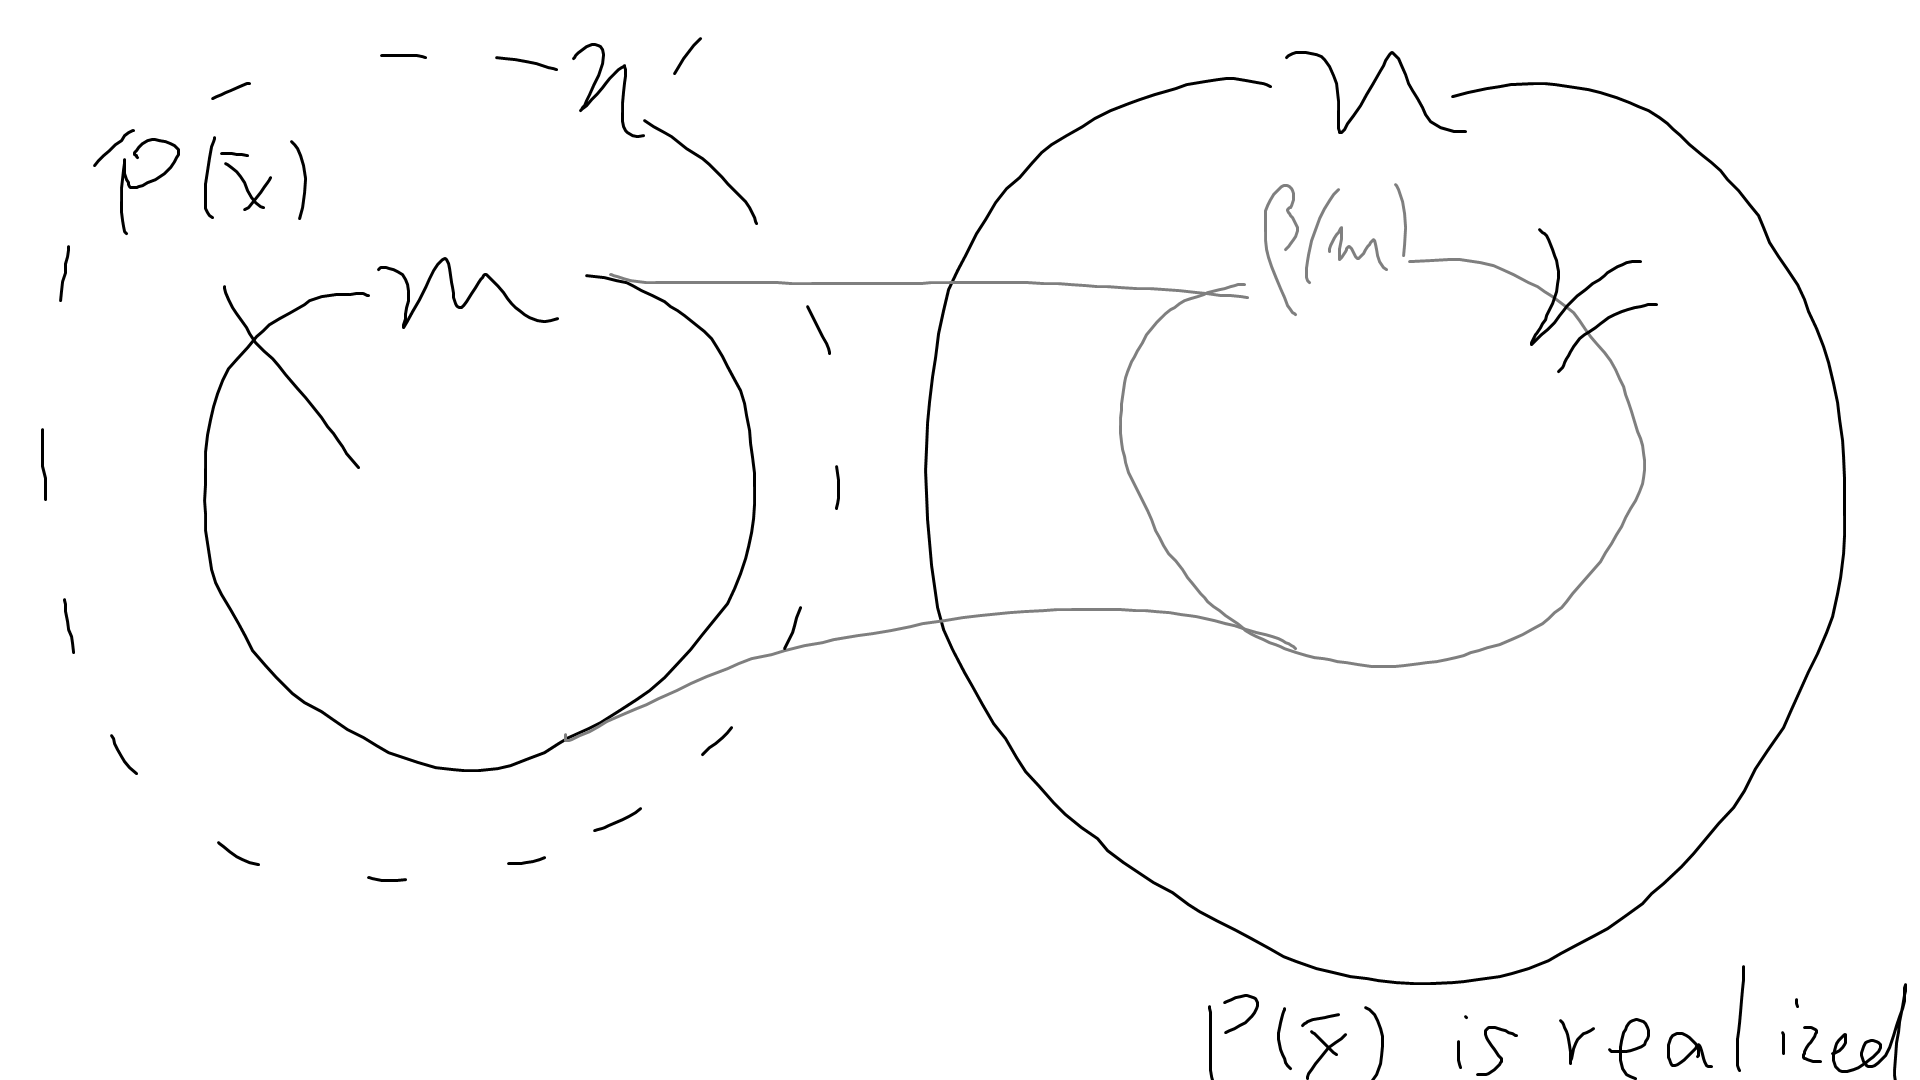
\includegraphics[scale=0.5]{image/Model_07.png}

    (Get $\mathcal{N}' \simeq \mathcal{N}$ s.t. $\mathcal{M} \preccurlyeq \mathcal{N}'$, $\mathcal{M} \simeq \beta(\mathcal{M})$.)
\end{proof}

\begin{thm} (5.12, Upward L$\ddot{o}$wenheim-Skolem theorem)\\
    (See part II Logic and Set theory for the (countable?) case)\\
    Let $\mathcal{M}$ be s.t. $|\mathcal{M}| \geq \omega$. Then for any $\lambda \geq |\mathcal{M}| + |L|$, there is $\mathcal{N}$ s.t. $\mathcal{M} \preccurlyeq \mathcal{N}$ with $|\mathcal{N}| = \lambda$.
    \begin{proof}
        Let $\bar{x} = \bra x_i: i < \lambda \ket$ a tuple of distinct variables.\\
        Let $p(\bar{x}) = \{x_i \neq x_j: i < j < \lambda\}$. Then $p(\bar{x})$ is finitely consistent in $\mathcal{M}$. So by theorem (5.11), $p(\bar{x})$ is realized in some $\mathcal{N}$ that is an elementary extension of $\mathcal{M}$, and $|\mathcal{N}| \geq \lambda$.\\
        Then by downward L-S theorem (3.11) we could have $|\mathcal{N}| = \lambda$.
    \end{proof}
\end{thm}

\newpage

\section{Saturation}

\begin{defi} (6.1)\\
    Let $\lambda$ be an infinite cardinal, let $|\mathcal{M}| \geq \omega$. Then $\mathcal{M}$ is \emph{$\lambda$-saturated} if $\mathcal{M}$ realizes every type $p(x)$ (with one free variable) such that:\\
    (i) $p(x)$ has parameters in $A \subseteq \mathcal{M}$ and $|A| < \lambda$;\\
    (ii) $p(x)$ is finitely consistent in $\mathcal{M}$.\\
    We say $\mathcal{M}$ is \emph{saturated} if it is $|\mathcal{M}|$-saturated.
\end{defi}

Question: can $\mathcal{M}$ be $\lambda$-saturated if $\lambda > |\mathcal{M}|$? If so, $\mathcal{M}$ would satisfy f.s. types in $L(M)$.\\
(Hint: we could use $p(x) = \{x \neq a_i: i < |\mathcal{M}|\}$ where $\bra a_i: i<|\mathcal{M}| \ket$ enumerates $\mathcal{M}$. This could not be satisfiable.)

---Lecture 10---

\begin{defi} (6.2)\\
    Let $\mathcal{M}$ be an $L$-structure, $A \subseteq M$, $\bar{b}$ a tuple of in $M$, possibly infinite.\\
    The type of $\bar{b}$ over $A$ is the following $L(A)$-type:
    $$tp_\mathcal{M}(\bar{b}/A) = \{\phi(\bar{x}) \in L(A): \mathcal{M} \vDash \phi(\bar{b})\}$$
    (i.e. all the $L(A)$-formulas that, when plugged in $\bar{b}$, can be implied by $\mathcal{M}$).\\
    $\mathcal{M}$ is often omitted if it's clear from the context.
\end{defi}

\begin{rem} (6.3)\\
    (i) $tp_{\mathcal{M}} (\bar{b}/A)$ is complete, i.e. for every $L(A)$ formula $\phi(\bar{x})$, either $\phi(\bar{x}) \in tp(\bar{b}/A)$ or $\neg\phi(x) \in tp(\bar{b}/A)$ (clear).\\
    (ii) If $\mathcal{M} \preccurlyeq\mathcal{N}$, then for $A \subseteq M$, and $\bar{b}$ a tuple,
    $$tp_\mathcal{M}(\bar{b}/A) = tp_\mathcal{N}(\bar{b}/A)$$
    (elementary embeddings preserve truth of formulas.)
\end{rem}

\begin{fact} (6.4, elementary maps and types)\\
    Recall definition (4.10):\\
    (i) If $f:A \subseteq \mathcal{M} \to \mathcal{N}$ is a (partial) elementary map, then in particular, $f$ preserves $L$-sentences, so $\mathcal{M} \equiv \mathcal{N}$.\\
    (ii) If $\mathcal{M} \equiv \mathcal{N}$, then $\phi$, the empty map, \emph{is} an elementary map (only required to preserve sentences).\\
    (iii) If $f:A \subseteq \mathcal{M} \to \mathcal{N}$ is elementary, and $\bar{a}$ is an enumeration of $A=\dom(f)$, then (obviously, $\phi$ denotes the empty set here)
    $$tp(\bar{a}/\phi) = tp(f(\bar{a})/\phi)$$
    More generally: if $f:\mathcal{M} \to \mathcal{N}$ (we'll stop writing $f:A \subseteq \mathcal{M} \to \mathcal{N}$ for elementary maps now) is elementary and there is $A\subseteq M \cap N$ s.t. $A \subseteq \dom(f)$, $f|_A = id$ ($f$ fixes $A$ pointwise), then for every tuple $\bar{b}$ in $\dom(f)$,
    $$tp_\mathcal{M} (\bar{b}/A) = tp_\mathcal{N} (f(\bar{b}),A)$$

    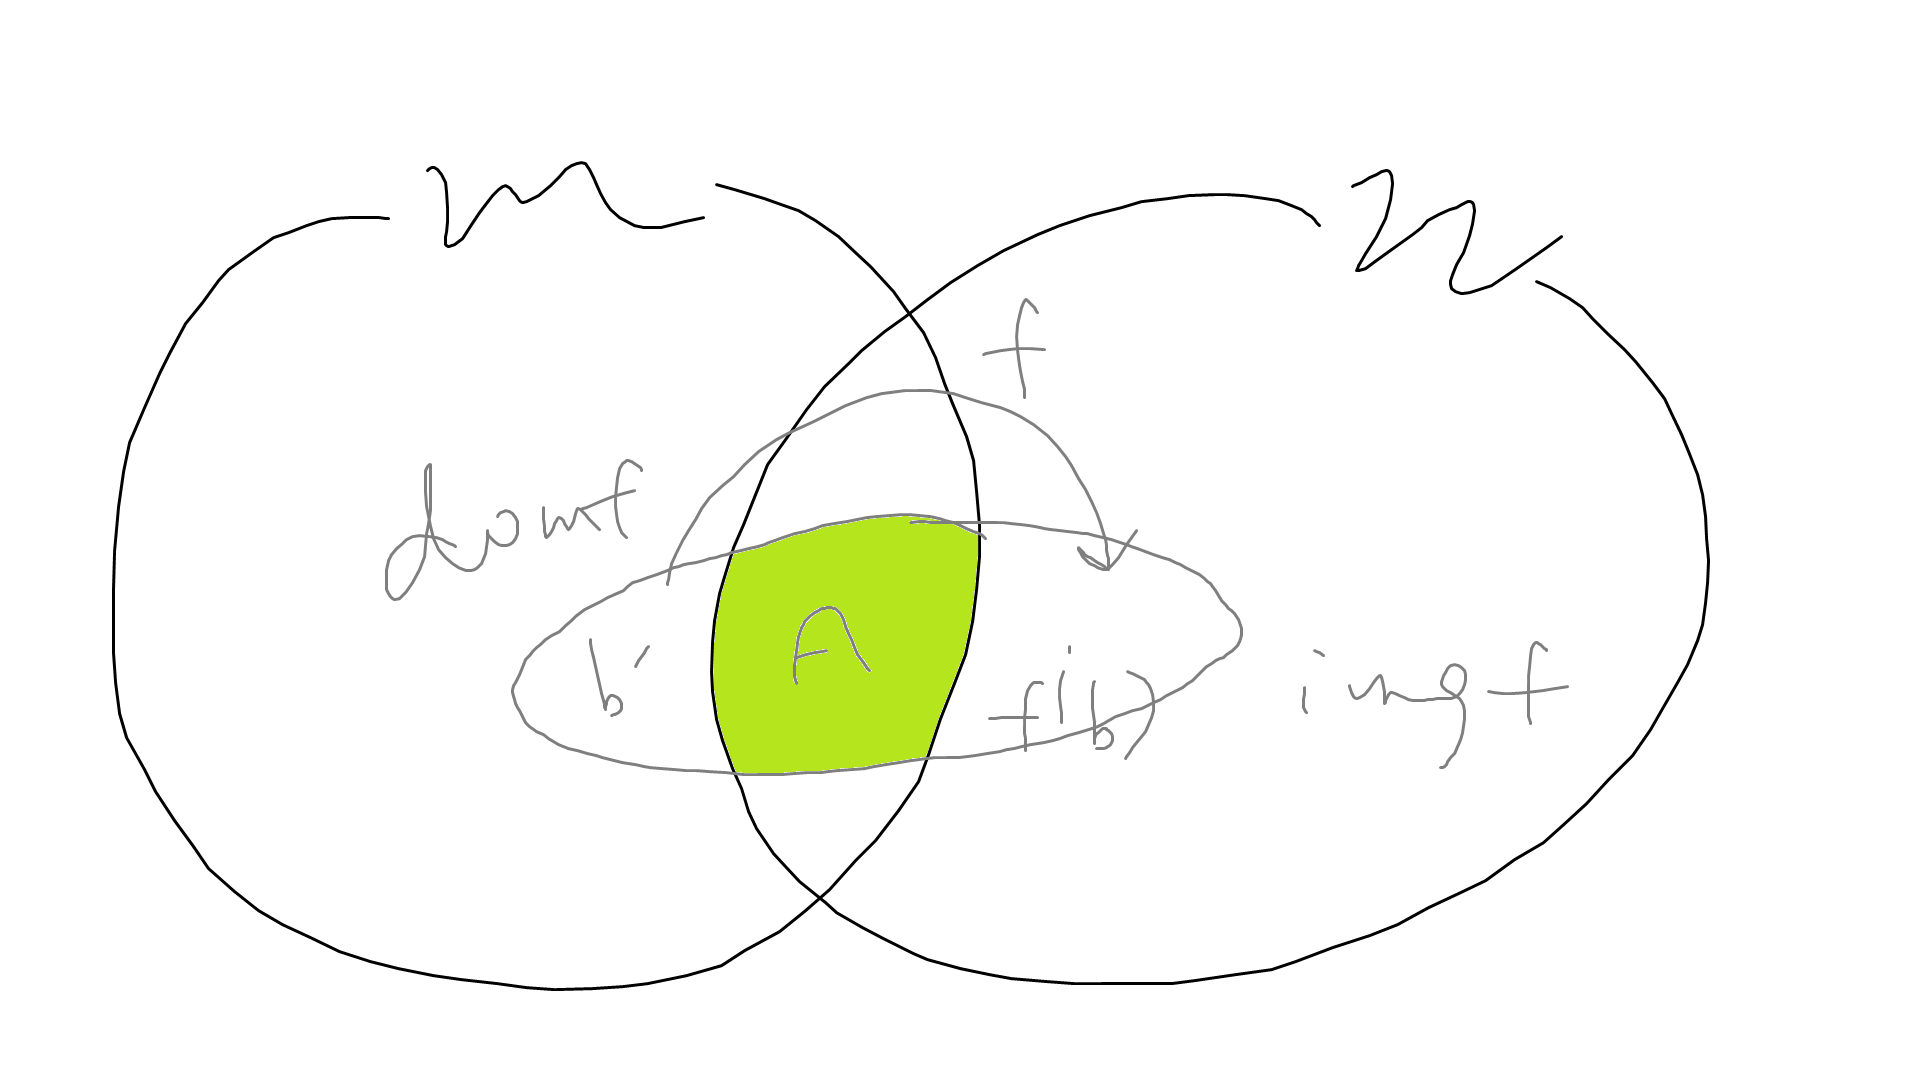
\includegraphics[scale=0.5]{image/Model_08.png}

    (iv) Let $\bar{a}$ enumerate $A \subseteq M$, $A=\dom(f)$ where $f:\mathcal{M} \to \mathcal{N}$ is elementary.\\
    Let $p(\bar{x},\bar{a})$ be a type in $L(A)$ that is finitely satisfiable in $\mathcal{M}$.\\
    Then $p(\bar{x},f(\bar{a}))$ is finitely satisfiable in $\mathcal{N}$: with massive abuse of notations, let $\{\phi_1(\bar{x},\bar{a}),...,\phi_n(\bar{x},\bar{a})\} \subseteq p(\bar{x},\bar{a})$.\\
    By f.s. of $p(\bar{x},\bar{a})$, $\mathcal{M} \vDash \exists \bar{x} \bigwedge_{i=1}^n \phi_i(\bar{x},\bar{a})$.\\
    Then $\mathcal{N} \vDash \exists \bar{X} \bigwedge_{i=1}^n \phi_i(\bar{x},f(\bar{a}))$ by elmentarity of $f$.\\
    (Does $p(\bar{x},\bar{a})$ satisfiable in $\mathcal{M}$ imply $p(\bar{x},f(\bar{a}))$ satisfiable in $\mathcal{N}$? The answer is no -- this doesn't hold in the infinite case.)
\end{fact}

(Note that we haven't really discussed about the existence of saturated models. The general result is that given any model with size $\lambda$ we could extend it elementarily to a model that is $\lambda^+$ saturated, but we'll have no control over the size of the extended model unless we assume some more subtle things (Lecturer was unsure of that)).

\begin{thm} (6.5)\\
    Let $\mathcal{N}$ be s.t. $|\mathcal{N}| \geq \lambda \geq |L|+\omega$. The following are equivalent:\\
    (i) $\mathcal{N}$ is $\lambda$-saturated;\\
    (ii) if $\mathcal{M} \equiv \mathcal{N}$, $b \in M$ and $f:\mathcal{M} \to \mathcal{N}$ partial elementary s.t. $|\dom f| < \lambda$, then there is partial elementary $\bar{f} \supseteq f$ such that $b \in \dom(\bar{f})$;\\
    (iii) If $p(\bar{z})$ is an $L(A)$-type where $|\bar{z}| \leq \lambda$, and $|A| < \lambda$ and $p(\bar{z})$ is finitely satifiable in $\mathcal{N}$, then $p(\bar{z})$ is satisfiable in $\mathcal{N}$.
    \begin{proof}
        (i) $\implies$ (ii): Let $f:\mathcal{M} \to \mathcal{N}$ be as in (ii), and let $b \in M$. The idea is the following: look at the type of $b$ over $M$, and then prove that the corresponding type in $\mathcal{N}$ is realized in $\mathcal{N}$.\\
        Let $\bar{a}$ be an enumeration of $\dom(f)$, so $|\bar{a}|<\lambda$. Let $p(x/\bar{a}) = tp_\mathcal{M} (b/\bar{a})$.

        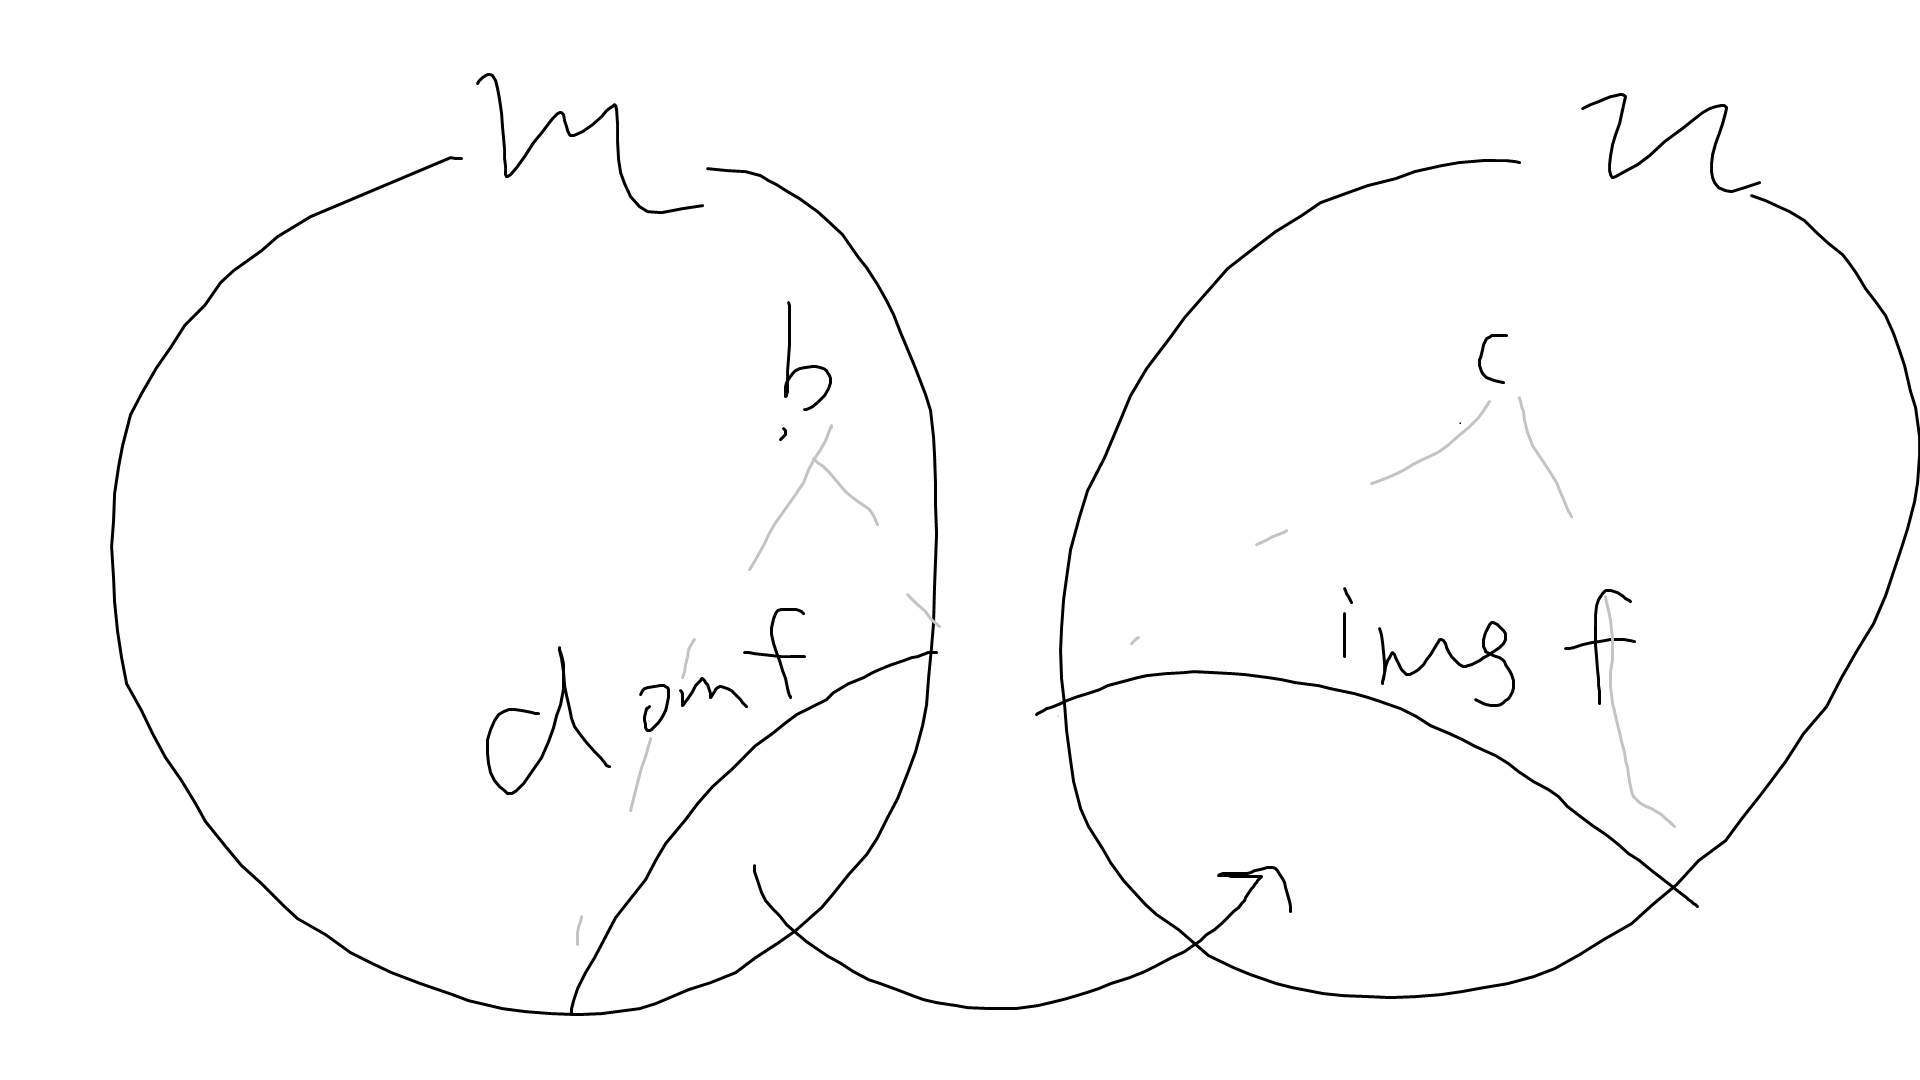
\includegraphics[scale=0.5]{image/Model_09.png}

        Then $p(x/\bar{a})$ is finitely satisfiable in $\mathcal{M}$, hence $tp(x/f(\bar{a}))$ is f.s. in $\mathcal{N}$ (6.4 (iv)).\\
        Since $|f(\bar{a})| < \lambda$ and $\mathcal{N}$ is $\lambda$-saturated, $tp(x/f(\bar{a}))$ is realized in $\mathcal{N}$ by some $c$.\\
        Then $f \cup \{\bra b,c\ket \}$ is the required extension.\\
        ($\mathcal{M} \vDash \phi(b,\bar{a}) \iff \mathcal{N} \vDash \phi(c,f(\bar{a}))$, so $f$ preserves the truth).\\
        (ii) $\implies$ (iii): (idea?: Let $p(\bar{z})$ be as in (iii), $p(\bar{z})$ is f.s. in $\mathcal{N}$. Then by (5.11), $p(\bar{z})$ is realized in some elementary extension $\mathcal{M}'$ of $\mathcal{N}$, by some tuple $\bar{a}$ (where $|\bar{a}| = |\bar{z}|$).\\
        But now we can shrink $|\mathcal{M}'|$ by downward L-S theorem: there is $\mathcal{M} \preccurlyeq\mathcal{M}'$ such that $A \cup \bar{a} \subseteq M$, where $A$ is the parameter set of the type.)

        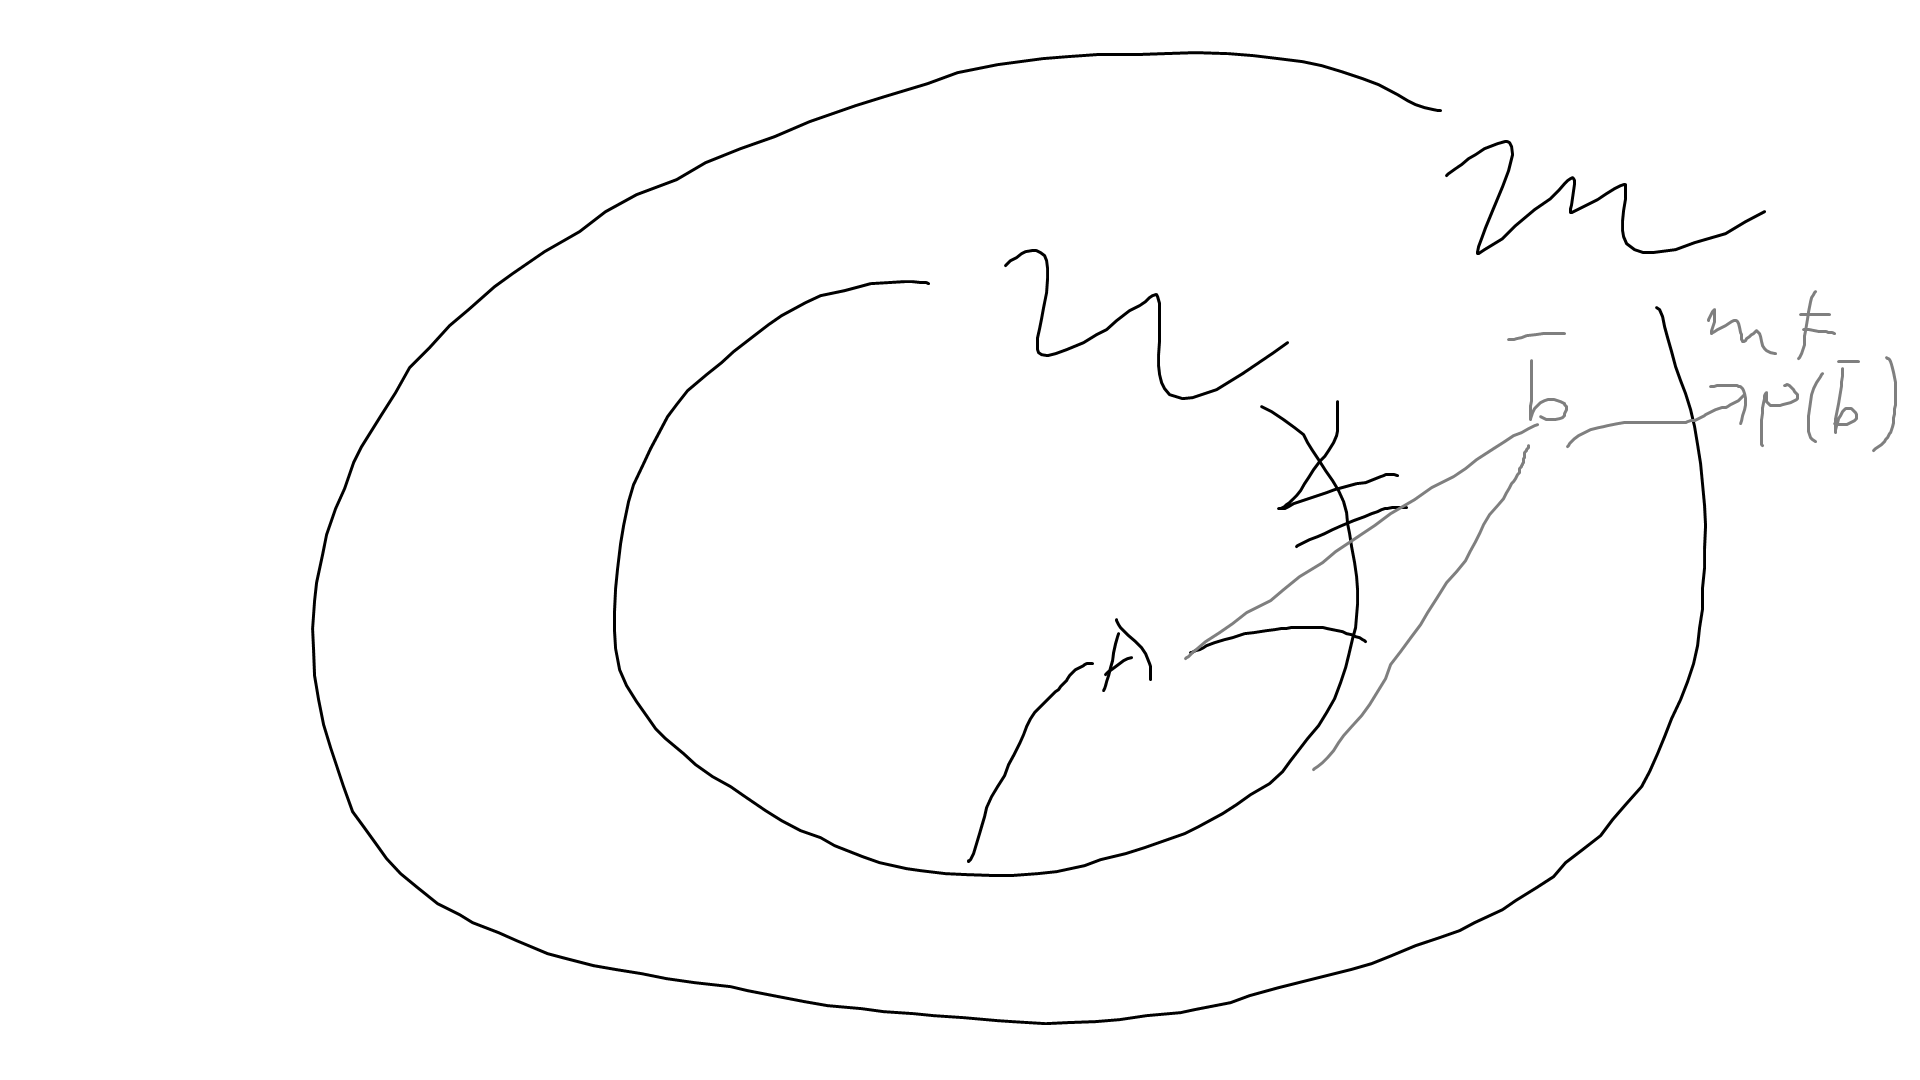
\includegraphics[scale=0.5]{image/Model_10.png}
        
        ---Lecture 11---

        Let $p(\bar{z})$ be as in (iii), $\mathcal{M}$ is s.t. $\mathcal{N} \preccurlyeq\mathcal{M}$ and $\mathcal{M} \vDash p(\bar{b})$. The identity map $id_A:\mathcal{M} \to \mathcal{N}$ is partial elementary.\\
        Idea: build $\bra f_i:i < |\bar{b}| \ket$ of $p$ elementary maps. Then $\cup f_i$ is partial elementary, and $\bar{b} \in \dom \cup_{i < |\bar{a}|} f_i$.\\
        Let $f_0 = id_A$. At stage $i+1$, use (ii) to put $b_i$ in $\dom (f_{i+1})$.\\
        At limit stages $\mu < \lambda$, let $f_\mu = \cup_{i < \mu} f_i$.\\
        Then $f(\bar{b})$ satisfies $p(\bar{z})$ in $\mathcal{N}$.

        (iii) $\implies$ (i) is trivial.
    \end{proof}
\end{thm}

\begin{coro} (6.6)\\
    If $\mathcal{M}$ and $\mathcal{N}$ are saturated, and $\mathcal{M} \equiv \mathcal{N}$, and $|\mathcal{M}| = |\mathcal{N}|$, then every elmentary map $f:\mathcal{M} \to \mathcal{N}$ extends to an isomorphism.\\
    In particular, these two structures are isomorphic (since the empty map $\phi$ is an elementary map).
    \begin{proof}
        Use theorem 6.5(ii) to extend $f:\mathcal{M} \to \mathcal{N}$ to an isomorphism by back-and-forth (similar to that in random graphs), taking unions at limit stages.
    \end{proof}
\end{coro}

\begin{coro} (6.7)\\
    Models of $T_{dlo}$ and $T_{rg}$ are $\omega$-saturated.
    \begin{proof}
        In chapter 4 we proved that we can do one point extensions for partial elmentary maps for both of the cases (4.3 and 4.17).\\
        So $(\Q,<)$ $\omega$-saturated.\\
        Is $(\R,<)$ $\omega_1$-saturated? No -- for example, the type $p(x):= \{x>q: q \in \Q\}$ is not realized).
    \end{proof}
\end{coro}

\begin{defi} (6.8)\\
    An isomorphism $\alpha:\mathcal{N} \to \mathcal{N}$ is called an \emph{automorphism}.\\
    The automorphism of $\mathcal{N}$ form a group denoted by $\Aut(\mathcal{N})$.\\
    If $A \subseteq N$, then we write $\Aut(\mathcal{N}/A)$ for the subgroup of $\Aut(\mathcal{N})$ that fixes $A$ pointwise, i.e. $\{\alpha \in \Aut(\mathcal{N}):\alpha|_A = id\}$.
\end{defi}

\begin{defi} (6.9\footnote{In some texts the definition of this is a bit different -- sometimes they use $\lambda^+$-universality for our $\lambda$-universality here. Homogeneity is sometimes called \emph{strong homogeneity}. \emph{Ultrahomogeneity} concerns partial embeddings instead of (partial) elementary maps.})\\
    (i) An $L$-structure $\mathcal{N}$ is $\lambda$-universal if for every $\mathcal{M} \equiv \mathcal{N}$ s.t. $|\mathcal{M}| \leq \lambda$, there is elementary embedding $\beta:\mathcal{M} \to \mathcal{N}$.\\
    In particular, $\beta$ would be an isomorphism between $\mathcal{M}$ and its image in $\mathcal{N}$, i.e. $\mathcal{N}$ contains a copy of $\mathcal{M}$.\\
    $\mathcal{N}$ is \emph{universal} if it is $|\mathcal{N}|$-universal.\\
    (ii) $\mathcal{N}$ is \emph{$\lambda$-homogeneous} if every elementary map $f:\mathcal{N} \to \mathcal{N}$ s.t. $|f|<\lambda$ extends to an automorphism of $\mathcal{N}$.
\end{defi}

\begin{thm} (6.10)\\
    Let $\mathcal{N}$ be s.t. $|\mathcal{N}| \geq |L|+\omega$. The following are equivalent:\\
    (i) $\mathcal{N}$ is saturated;\\
    (ii) $\mathcal{N}$ is universal and homogeneous.
    \begin{proof}
        (i) $\implies$ (ii): Assume $\mathcal{N}$ is saturated, let $\mathcal{M} \equiv \mathcal{N}$ and s.t. $|\mathcal{M}| \leq |\mathcal{N}|$.\\
        Then let $\bar{a}$ enumerate $M$, let $p(\bar{x}) = tp(\bar{a}/\phi)$. Then $p(\bar{x})$ is f.s. in $\mathcal{M}$.\\
        We claim that $p(\bar{x})$ is also f.s. in $\mathcal{N}$: let $\{\phi_1(\bar{x}),...,\phi_m(\bar{x})\}$, so $\mathcal{M} \exists \bar{x} \bigwedge_{i=1}^n \phi_i(\bar{x})$; but note that this is a sentence, so $\mathcal{N} \vDash \exists \bar{x} \bigwedge \phi_i(\bar{x})$ as well.\\
        Now since $|\bar{x}| \leq |\mathcal{N}|$, $n$ realizes $p(\bar{x})$ since it's saturated (6.5 (iii)). Homoegeneity follows from (6.6).

        Conversely, we show that if $\mathcal{M} \equiv \mathcal{N}, b \in M$, $f:\mathcal{M} \to \mathcal{N}$ elementary s.t. $|f| < |\mathcal{N}|$, then there is $\hat{f} \supseteq f$ elementary and contains $b$ in its domain (i.e. we can extend $f$ to be defined on $b$).

        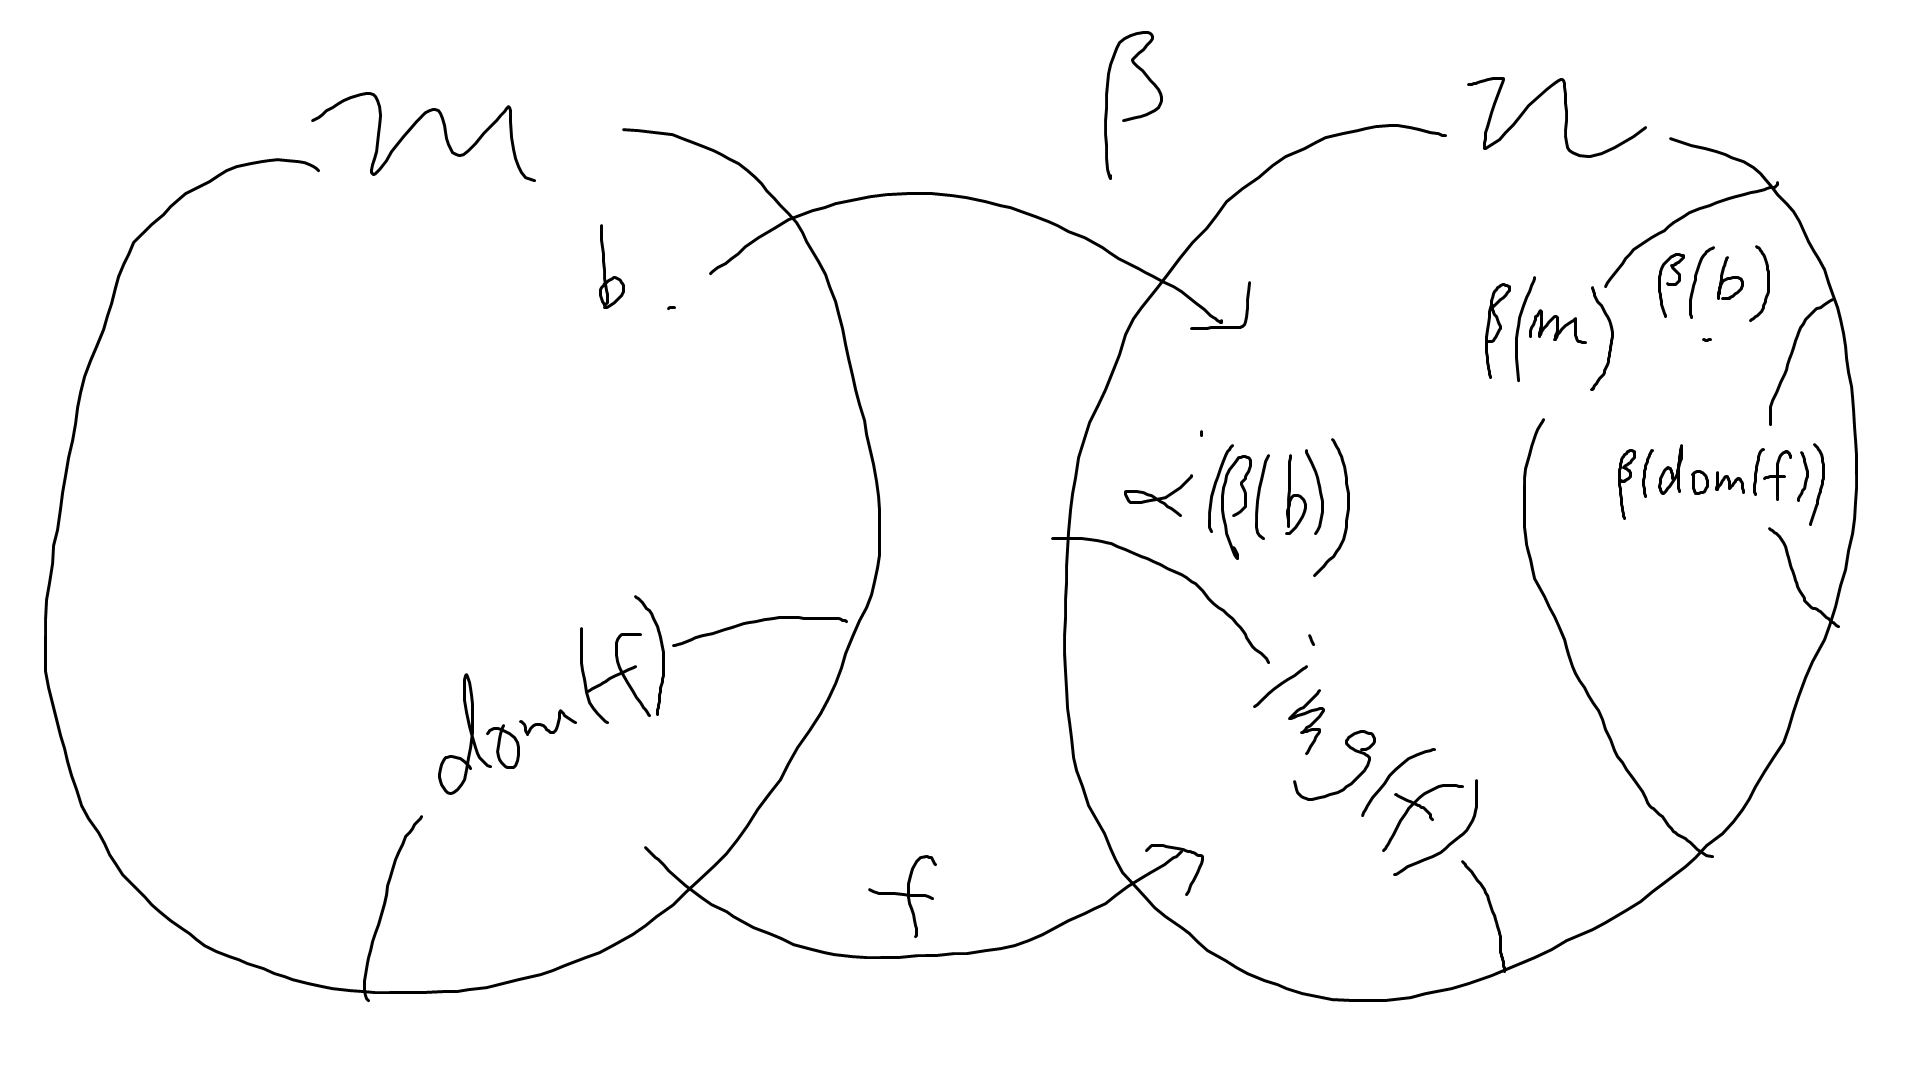
\includegraphics[scale=0.5]{image/Model_11.png}

        (Find?) $\alpha \in \Aut(\mathcal{N})$ extending $\beta(\dom(f)) \to img(f)$.

        (see lecturer's scanned notes for more details -- tbd.)
    \end{proof}
\end{thm}

\begin{defi} (6.11)\\
    Let $\bar{a}$ be a tuple in $\mathcal{N}$ and $A \subseteq N$. The \emph{orbit of $\bar{a}$} over $A$ is the set
    $$O_\mathcal{N} (\bar{a}/A) = \{\alpha(\bar{a}):\alpha \in \Aut(\mathcal{N}/A)\}$$
    If $\phi(\bar{x})$ is an $L(A)$-formula, then
    $$\phi(\mathcal{N}) := \{\bar{a} \in N^{|\bar{x}|}:\mathcal{N} \vDash \phi(\bar{a})\}$$
    (called the set defined by $\phi(\bar{x})$).\\
    A set is definable over $A$ if it is defined by some $L(A)$-formula.
\end{defi}

There are analogous notions of a type defining a set, and a set being type-definable -- lecturer will say more about this next time.

---Lecture 12---

\begin{rem} (6.12)\\
    If $\bar{a}$ and $\bar{b}$ are tuples in $\mathcal{N}$ and $|\bar{a}| = |\bar{b}|$, and $A \subseteq N$, then the following are equivalent:\\
    (i) $tp_\mathcal{N}(\bar{a}/A) = tp_\mathcal{N}(\bar{b})/A$;\\
    (ii) $\{\bra a_i,b_i\ket : i<|\bar{a}|\} \cup id_A$ is an elementary map.
\end{rem}

\begin{prop} (6.13)\\
    Let $\mathcal{N}$ be $\lambda$-homogeneous, $A \subseteq \mathcal{N}$ s.t. $|A| < \lambda$. Let $\bar{a}$ be a tuple in $\mathcal{N}$ s.t. $|\bar{a}| < \lambda$. Then
    $$O_\mathcal{N} (\bar{a}/A) = p(\mathcal{N})$$
    where $p(\bar{x}) = tp_\mathcal{N}(\bar{a}/A)$.
    \begin{proof}
        If $\alpha(\bar{a}) = \bar{b}$ where $\alpha \in \Aut(\mathcal{N} /A)$, then $tp_\mathcal{N}(\bar{A}/A) = tp_\mathcal{N}(\bar{b}/A)$.\\
        If $tp_\mathcal{N}(\bar{b}/A) = tp_\mathcal{N}(\bar{a}/A)$, then $\{\bra a_i,b_i:i < |\bar{a}| \} \cup id_A$ is elementary, and by homogeneigy it extends to $\alpha \in \Aut(\mathcal{N})$, and in particular, $\alpha \in \Aut (\mathcal{N} / A)$.
    \end{proof}
\end{prop}

\newpage

\section{The Monster Model}

Given a complete theory $T$ with an infinite model, we work in a saturated structure $U(\mathbb{M})$ that is a model of $T$ and is sufficiently large that any other model of $T$ we might be interested in is an elementary substructure of $U$.\\
($I$ is an expository device -- see Tent/Ziegler fo details -- also Marker(v?)).

\begin{defi} (7.1, terminologies and conventions)\\
    When working in $U$, \\
    $\bullet$ \emph{$\phi(\bar{x})$ holds} means $U \vDash \forall \bar{x} \phi(\bar{x})$;\\
    $\bullet$ \emph{$\phi(\bar{x})$ is consistent} means $U\vDash \exists \bar{x} \phi(\bar{x})$;\\
    $\bullet$ \emph{the type $p(\bar{x})$ is consistent/satisfiable} if $U \vDash \exists \bar{x} p(\bar{x})$;\\
    $\bullet$ a cardinality $\lambda$ is \emph{small} if $\lambda < |U|$ (we usually denote $|U|$ by $\kappa$).\\
    $\bullet$ a \emph{model} is $\mathcal{M} \preccurlyeq U$ s.t. $|\mathcal{M}|$ is small.

    Conventions:\\
    $\bullet$ tuples have small lengths (unless otherwise specified);\\
    $\bullet$ formulas have parameters in $U$;\\
    $\bullet$ types have parameters in small sets;\\
    $\bullet$ definable sets have the form $\phi(U)$ for some formula $\phi(\bar{x})$ in $L(U)$;\\
    $\bullet$ type definable sets have form $p(U)$ for some type $p(\bar{x},A)$ where $|A| < \kappa$;\\
    $\bullet$ Orbits and types of tuples are within $U$, so $tp(\bar{a}/A)$ means $tp_U(\bar{a}/A)$; $O(a/A)$ means $O_U(a/A)$;\\
    $\bullet$ if $p(\bar{x}),q(\bar{x})$ are types, we write, for example, $p(x) \to q(x)$ to mean $p(\mathcal{N}) \subseteq q(\mathcal{N})$ (think of $p(x)$ as \emph{infinite conjunction of formulas}).
\end{defi}

\begin{fact} (7.2)\\
    Let $p(\bar{x})$ be a satisfiable $L(A)$-type, $q(\bar{x})$ be a satisfiable $L(B)$-type such that $p(\bar{x}) \to \neg q(\bar{x})$, that is, $p(\bar{x})$ and $q(\bar{x})$ have no realizations in common.\\
    Then there are $\bigwedge_{i=1}^n \phi_i(\bar{x})$ where $\phi_i(\bar{x}) \in p(\bar{x})$, and $\bigwedge_{i=1}^m \psi_i(\bar{x})$ where $\psi_i(\bar{x}) \in q(\bar{x})$ s.t.
    $$\bigwedge_{i=1}^n \phi_i(\bar{x}) \to \neg (\bigwedge_{i=1}^m \psi_i(\bar{x}))$$
    \begin{proof}
        We know $p(\bar{x}) \cup q(\bar{x})$ is not realized in $U$. By saturation of $U$, this cannot be finitely satisfiable, i.e. there are $\{\phi_i(\bar{x}),...,\phi_n(\bar{x})\} \subseteq p(\bar{x})$, $\{\psi_1(\bar{x}),...,\psi_m(\bar{x})\} \subseteq q(\bar{x})$ such that the union is not satisfiable. Then 
        $$\bigwedge \phi_i(\bar{x}) \to \neg \bigwedge (\psi_i(\bar{x}))$$
    \end{proof}
\end{fact}

\begin{rem} (7.3)\\
    Let $\phi(U,\bar{b})$ (note that this notation defines a set, i.e. the set of $\bar{a}$ s.t. $\phi(\bar{a},\bar{b})$ holds, where $\bar{a}$ is of correct length with each component in $U$) be s.t. $\phi(\bar{x},\bar{z})$ is an $L$-formula, $\bar{b} \in U^{|\bar{z}|}$.\\
    If $\alpha \in \Aut(U)$, then
    \begin{equation*}
        \begin{aligned}
            \alpha[\phi(U,\bar{b})] &= \{\alpha(\bar{a}): \phi(\bar{a},\bar{b}),\bar{a} \in U^{|\bar{x}|}\}\\
            &= \{\alpha(\bar{a}):\phi(\alpha(\bar{a}),\alpha(\bar{b})),...\}\\
            &= \phi(U,\alpha(\bar{b}))
        \end{aligned}
    \end{equation*}
    So $\Aut(U)$ acts on the definable sets in a natural way (similarly for type-definable sets).
\end{rem}

\begin{defi} (7.4)\\
    A set $D \subseteq U^\lambda$ is invariant under $\Aut(U/A)$ (\emph{invariant over} $A$) if $\alpha(D) = D$ for every $\alpha \in \Aut(U/A)$.\\
    Equivalently, for all $\bar{a} \in D$, $O(a/A) \subseteq D$.\\
    If $\bar{a} \in D$, $q(\bar{x}) = tp(a/A)$ and $\bar{b} \vDash q(\bar{x})$, then $b \in D$.\\
    ($tp(\bar{b}/A) = tp(\bar{a}/A)$ and $\bar{b} \vDash q(\bar{x})$, so there's $\alpha \in \Aut(U/A)$ s.t. $\alpha(\bar{a}) = \bar{b}$ by homogeneity of $U$).\\
    Hence another equivalent formulation of invariance over $A$ is: for all $\bar{a} \in D$, if $\bar{b} \equiv_A \bar{a}$, then $\bar{b} \in D$.
\end{defi}

\begin{prop} (7.5)\\
    Let $\phi(\bar{x})$ be an $L(U)$-formula. The following are equivalent:\\
    (i) $\phi(\bar{x})$ is equivalent to some $L(A)$-formula $\psi(\bar{x})$;\\
    (ii) $\phi(U)$ is invariant over $A$.
    \begin{proof}
        (i) $\implies$ (ii) is clear (set-wise invariance);\\
        (ii) $\implies$ (i) This is the more interesting direction. Let $\phi(\bar{x},\bar{z})$ be an $L$-formula s.t. $\phi(U,\bar{b})$ is invariant over $A$ (for $\bar{b} \in U^{|z|}$).\\
        Let $q(\bar{z}) = tp(\bar{b}/A)$. If $\bar{c} \vDash q(\bar{z})$, then there is (by homogeneity), $\alpha \in \Aut (U/A)$ s.t. $\alpha(\bar{b}) = \bar{c}$. Then 
        $$\phi(U,\bar{b}) = \alpha(\phi(U,\bar{b})) = \phi(U,\bar{c})$$
        by invariance and (7.3) respectively. Hence $q(\bar{z}) \to \forall \bar{x} [\phi(\bar{x},\bar{z}) \leftrightarrow \phi(\bar{x},\bar{b})]$. By (an argument similar to 7.2) there is $\theta(\bar{z}) \in q(\bar{z})$ s.t. $\theta(\bar{z}) \to \forall \bar{x}[\phi(\bar{x},\bar{z}) \leftrightarrow \phi(\bar{x},\bar{z})]$.\\
        Then $\theta(\bar{z})$ is an $L(A)$-formula, and $\exists z [\theta(\bar{z}) \wedge \phi(\bar{x},\bar{z})]$ defines $\phi(U,\bar{b})$.
    \end{proof}
\end{prop}

---Lecture 13 to be typesetted---

\begin{defi} (7.6)\\
    An injective map $\rho:A \subset \mathcal{M} \to \mathcal{N}$ is a \emph{partial embedding} if for all tuples in $A=\dom\rho$, $\rho$ satisfies conditions (i)-(iii) in definition (1.5) (i.e. $\rho$ is an embedding $\dom \rho \to \im \rho$).
\end{defi}

\begin{prop} (7.7)\\
    Let $\phi(\bar{x})$ be an $L$-formula. The following are equivalent:\\
    (i) $\exists \psi(\bar{x})$, a quantifier free $L$-formula, s.t. $U \vDash \forall \bar{x}(\phi(\bar{x}) \iff \psi(\bar{x}))$;\\
    (ii) $\forall \rho$ a partial embedding $U \to U$, $\forall \bar{A} \in \dom \rho$, $\phi(\bar{a}) \iff \phi(\rho(\bar{a}))$.
\end{prop}

---Lecture 14---

Possible erratum to theorem (7.9) (iii) $\implies$ (ii): 
\begin{proof}
    Let $p:U \to U$ be a partial embedding. Consider $p_0 \subseteq p$, $p_0$ finite or small. Use property (iii) and saturation to extend $p_0$ to $\alpha \in \Aut(U)$ by back and forth.
\end{proof}

\begin{thm} (7.12)\\
    Let $A \subseteq U$, $a \in U$. The following are equivalent:\\
    (i) $a \in acl(A)$;\\
    (ii) $|O(a/A)| < \omega$ (orbit of $a$ under automorphisms of $A$ is finite);\\
    (iii) $a \in \mathcal{M}$ for any model $\mathcal{M}$ which contains $A$.
    \begin{proof}
        (i) $\implies$ (ii): If $a \in acl(A)$, then there is $L(A)$-formula $\phi(x)$ s.t. $\phi(a)$ and $|\phi(U)| < \omega$. But $\phi(U)$ is invariant over $A$, and so $O(a/A) \subseteq \phi(U)$, and so $|O(a/A)| < \omega$.\\
        (ii) $\implies$ (i): If $|O(a/A)| < \omega$, then $O(a/A)$ is definable, by $\vee_{i=1}^n x=a_i$ where $P(a/A) = \{a_1,...,a_n\}$. Also $O(a/A)$ is invariant over $A$. So by (7.5), there is an $L(A)$-formula $\phi(x)$ that defines $O(a/A)$.\\
        (i) $\implies$ (iii): Suppose $a \in acl(A)$, so there is $\phi(x)$, an $L(A)$-formula, s.t. there is $n \in \omega \setminus \{0\}$ that
        $$ (U\vDash) \phi(a) \wedge \exists^{\leq n} x \phi(x)$$
        (where the notation means \emph{there are at most $n$ solutions to}). Then by elementarity, $\exists^{\leq n} x \phi(x)$ holds in every $\mathcal{M} \supseteq A$, and the $n$ realizations of $\phi(x)$ in $U$ must coincide with the realizations in $\mathcal{M}$. Therefore $a \in \mathcal{M}$ (?).\\
        (iii) $\implies$ (i): Suppose $a \not\in acl(A)$, let $p(x) = tp(a/A)$. Then for $\phi(x) \in p(x)$, $|\phi(U)| \geq \omega$. Then by Sheet 2 Q8, $|p(U)| \geq \omega$. By an argument similar to the on in Q7, $|p(U)| = |U|$.

        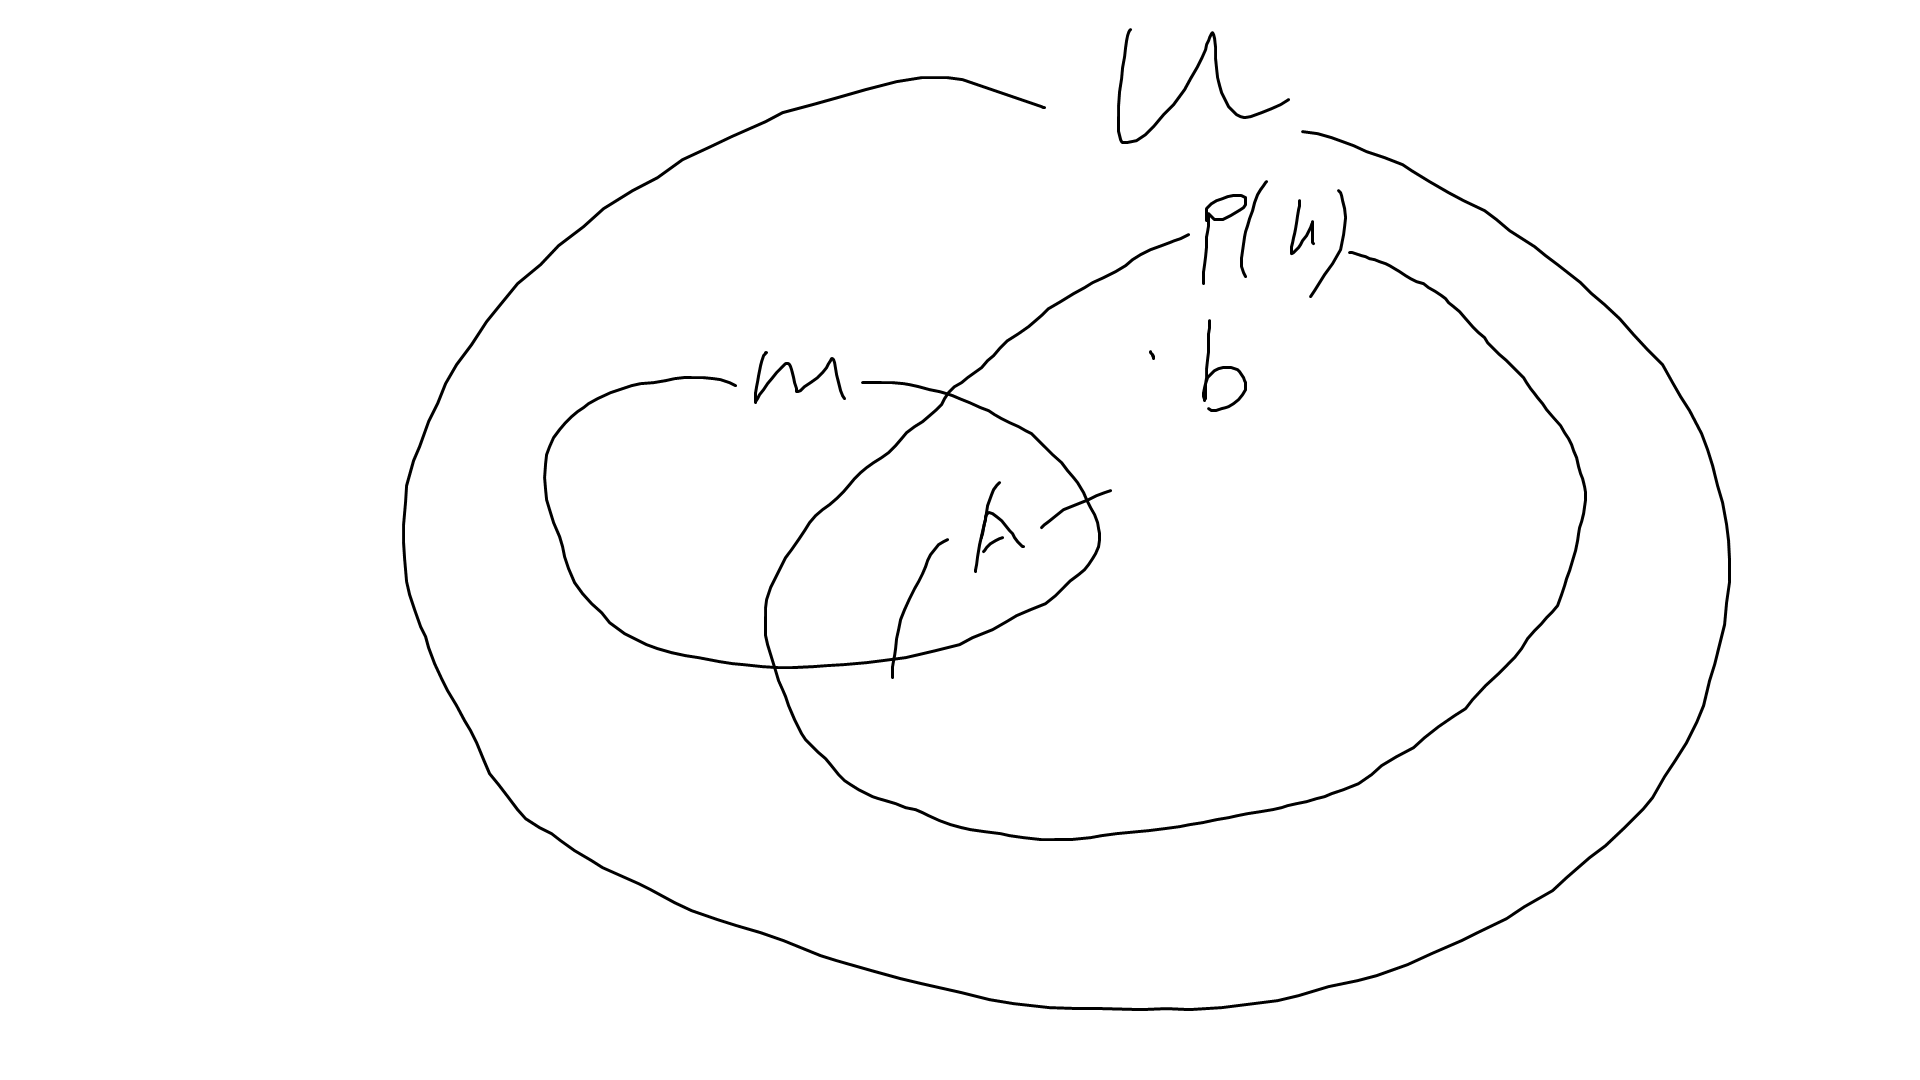
\includegraphics[scale=0.5]{image/Model_12.png}

        Let $\mathcal{M} \supset A$, Then $p(U) \setminus \mathcal{M} \neq \phi$. So there is $b \in p(U) \setminus \mathcal{M}$ Since $tp(a/A) = tp(b/A)$, there is $\alpha \in \Aut(U/A)$ s.t. $\alpha(b) = a$. But then $\alpha[\mathcal{M}]$ is a model that contains $A$, but it cannot contain $a$ as $a = \alpha(b)$ and $b \not\in \mathcal{M}$.
    \end{proof}
\end{thm}

\begin{prop} (7.13)\\
    Let $a \in U$, $A \subseteq U$. Then \\
    (i) if $a \in acl(A)$, then there is finite $A_0 \subseteq A$ s.t. $a \in acl(A_0)$;\\
    (ii) if $A \subseteq B$, then $acl(A) \subseteq acl(B)$;\\
    (iii) $acl(A) = acl(acl(A))$;\\
    (iv) $A \subseteq acl(A)$;\\
    (v) $acl(A) =\cap_{A \subseteq \mathcal{M}} \mathcal{M}$ (where $\mathcal{M}$ is any small elemntary substructure of $U$).
    \begin{proof}
        (iv) $a \in A$ is definable over $A$, hence algebraic.\\
        (iii) $acl(A) \subseteq acl(acl(A))$ by monotonicity (iv). For $\supseteq$, let $a \in acl(acl(A))$. By theorem (7.12), $a \in \mathcal{M}$ for every $\mathcal{M} \supseteq acl(A)$. But $acl(A) \subseteq \mathcal{M} \iff A \subseteq \mathcal{M}$, so in fact $a \in \mathcal{M}$ for every $\mathcal{M} \supseteq A$, i.e. $a \in acl(A)$.\\
        (v) follows directly from (7.12) (i) $\iff$ (iii).
    \end{proof}
\end{prop}

\begin{prop} (7.14)\\
    If $\beta \in \Aut(U)$, $A \subseteq U$, then 
    $$\beta[acl(A)] = acl(\beta[A])$$
    (Slogan (to make this more astounding): The operator $acl$ is a \emph{natural transformation} on $\Aut(U)$).
    \begin{proof}
        $\subseteq$: Let $a \in acl(A)$, let $\phi(x,\bar{z})$ be an $L$-formula s.t. $\phi(a,\bar{b})$ holds for $\bar{b}$ in $A$, and $|\phi(U,\bar{b})| < \omega$. Then $\phi(\beta(a),\beta(\bar{b}))$ holds, $|\phi(U,\beta(\bar{b}))| < \omega$, and so $\beta(a)$ is algebraic over $\beta[\bar{b}]$.\\
        The same proof with $\beta^{-1}$ in place of $\beta$ and $\beta[A]$ in place of $A$ show $\supseteq$.
    \end{proof}
\end{prop}

\newpage

\section{Strongly minimal theories}

\begin{defi} (8.1)\\
    Let $\mathcal{M}$ be a structure. $A\subseteq M$ is \emph{cofinite} if $M \setminus A$ is finite.
\end{defi}

\begin{rem} (8.2)\\
    Finite and cofinite sets are definable (from now on we always mean definable with parameters) in every structure.\\
    In this chapter, we'll look at structures where these are the only definable sets.
\end{rem}

\begin{defi} (8.3)\\
    A structure $\mathcal{M}$ is \emph{minimal} if all its definable subsets are finite or cofinite.\\
    Unfortunately (as we could expect), this is not definable in first-order logic. So we'll introduce a stronger notion: $\mathcal{M}$ is \emph{strongly minimal} if it is minimal and all its elementary extensions are minimal.\\
    If $T$ is a consistent theory without finite models, $T$ is \emph{strongly minimal} if for every formula $\phi(x,\bar{z})$, there is $n \in \omega \setminus 0$ s.t.
    $$T \vdash \forall \bar{z} [\exists^{\leq n} x \phi(x,\bar{z}) \vee \exists^{\leq n} x \neq \phi(x,\bar{z})]$$
\end{defi}

\begin{eg}
    $L=\{E\}$ where $E$ is binary, let $\mathcal{M}$ be the $L$-structure where $E$ is an equivalence relation with exactly one class of size $n$ for all $n \in \omega$, and no infinite classes.\\
    We can show $\mathcal{M}$ is minimal (can only say $\wedge$ of things like $x$ is in the same class as $a$).\\
    There is $\mathcal{N} \succcurlyeq \mathcal{M}$ where $\mathcal{N}$ has an infinite class. Then if the equivalence class of $a \in \mathcal{N}$ is infinite, the set defined by $E(x,a)$ is infinite/coinfinite.
\end{eg}

\begin{rem}
    Strongly minimal theories have monster models.
\end{rem}

From now on, we'll assume by default $T$ is strongly minimal, complete, and has an infinite model.

\begin{defi} (8.4)\\
    Let $a \in U$ a monster model of $T$, $B \subseteq U$. Then $a$ is \emph{independent from $B$} if $a \not\in acl(B)$.\\
    The set $B$ is \emph{independent} if for all $a \in B$, $a \not\in acl(B\setminus\{a\})$.
\end{defi}

---Lecture 15---

Reminder: optional non-examinable lecture on Monday 26 (on saturated models).

Thursday 17 January: third example class (2-3 pm).

\begin{eg}
    Consider \emph{Vector spaces}: Fix an infinite field $K$; $L_K = \{+,-,\mathbf{0},\{\lambda\}_{\lambda \in K}\}$ where $\lambda$ are unary functions (for scalar multiplications).\\
    Let $T_{VSK}$ be the theory of vector spaces over $K$, which includes:\\
    $\bullet$ axioms in $\{+,-,\mathbf{0}\}$ for abelian group;\\
    $\bullet$ axiom schemata for scalar multiplication: $\forall xy[\lambda(x+y)=\lambda x+\lambda y]$ for each $\lambda \in K$, where by $\lambda x$ means $\lambda(x)$;
    $\bullet$ $\forall x [1x = x]$ where $1$ is in scalar in $K$;\\
    $\bullet$ $\exists x[x \neq \mathbf{0}]$.

    Fact: $T{VSK}$ is complete and has q.e..\\
    Atomic formulas: equality of linear combinations;\\
    Atomic formula in one variable and with parameters is equivalent to something of the form $\lambda x = a$, so atomic formulas in one variable define singletons.\\
    Quantifier-free formulas in one variable and with parameters define sets that are either finite or cofinite.\\
    By q.e., $T_{VSK}$ is strongly minimal.\\
    Also: $acl(A) = \bra A \ket$ the linear span of $A$, so $a$ is independent from $A$ if it is not a linear combination of elements in $A$, and a set $A$ is independent if it is linearly independent (that probably explains the name).

    Now consider \emph{Fields}: In the language $L_{ring} =\{+,\cdot,-,0,1\}$, we use ACF (algebraic closed field) to denote the theory that includes:\\
    $\bullet$ axioms for abelian group in $\{+,-,0\}$;\\
    $\bullet$ axioms for multiplicative monoid $\{\cdot,1\}$;\\
    $\bullet$ distributivity: $\forall xyz [x \cdot (y+z) = x \cdot y + x \cdot z]$;\\
    $\bullet$ multiplicative inverse: $\forall x [x = 0 \vee \exists y ( x \cdot y) = 1]$;\\
    $\bullet$ $0 \neq 1$;\\
    The above characterizes a field; for algebraic closedness, we further add\\
    $\bullet$ axioms for algebraic closure: for all $n$, $\forall x_0,...,x_n \exists y [x_n y^n + ... + x_0 = 0]$.

    It can be proved that ACF is q.e., but is not complete (because it doesn't determine the characteristic of the field). If $\chi_p \equiv \underbrace{1+1+...+1}{p \text{ times}} = 0$, then ACF + $\{\chi_p\}$ = $ACF_p$, which is complete and has q.e..\\
    By adding $\{\neg \chi_n: n \in \omega\}$ to ACF, we get a theory $ACF_0$ which is also complete and q.e..\\
    Atomic formulas with parameters are polynomial equations; an atmoic formula with one variable (and parameters in $A$) is equivalent to $p(x) = 0$ where $p(x)$ is a polynomial in the subfield generated by $A$. So such atomic formulas define finite sets (solution sets), and q.f. formulas define finite or cofinite sets, and so by q.e., $ACF_p$ ($ACF_0$) is strongly minimal.\\
    If $a \in \mathcal{M} \vDash ACF_p$, $A \subseteq \mathcal{M}$, $a \in acl(A)$ is algebraic over the field generated by $A$.
\end{eg}

If $a \in U$, $A \subseteq U$, remember that $a$ is independent from $A$ if $a \not\in acl(A)$.\\
Notation: we write $acl(a,B)$ for $acl(\{a\} \cup B)$, and $acl(B \setminus a)$ for $acl(B \setminus \{a\})$.

\begin{thm} (8.5)\\
    Let $B \subseteq U$, and $a,b \not\in acl(B)$ ($a,b \in U \setminus acl(B)$).\\
    Then $b \in acl(a,B) \iff a \in acl(b,B)$.
    \begin{proof}
        Let $a,b \not\in acl(B)$. Assume $b \not\in acl(a,B)$ and $a \in acl(b,B)$.\\
        Then we have some $\phi(x,y)$, an $L(B)$-formula, s.t. for some $n$, $\phi(a,b) \wedge \exists^{\leq n} x \phi(x,b)$.\\
        Since $b \not\in acl(a,B)$, the formula $\psi(a,y) \equiv \phi(a,y) \wedge \exists^{\leq n} x \phi(x,y)$ is s.t. $|\psi(a,U)| \geq \omega$.\\
        Hence $|\psi(a,U)| = |U|$. By strong minimality, $|\neg \psi(a,U)| < \omega$. By cardinality consideration, if $\mathcal{M} \supseteq B$, then $\mathcal{M}$ contains $c$ s.t. $\psi(a,c)$. But then $a \in acl(c,B)$, so $a \in \mathcal{M}$. Therefore $a$ is in all models containing $B$; so $a \in acl(B)$, contradiction by (7.12).
    \end{proof}
\end{thm}

\begin{defi} (8.6)\\
    Let $B \subseteq C \subseteq U$. Then $B$ is a \emph{basis} of $C$ if\\
    (i) $B$ is independent;\\
    (i) $C \subseteq acl(B)$ (or equivalently, $acl(B) = acl(C)$).
\end{defi}

\begin{lemma} (8.7)\\
    If $B$ is indenepdent and $a \not\in acl(B)$, then $\{a\} \cup B$ is independent.\\
    \begin{proof}
        Let $A \not\in acl(B)$, and suppose (for contradiction) that $\{a\} \cup B$ is not independent. Then there is $b \in B$ s.t. $b \in acl(a,B \setminus b)$. But then $b \not\in acl(B \setminus b)$; since $a \not\in acl(B)$, we have $a \in acl(b,B\setminus b) = acl(B)$. Contradiction.
    \end{proof}
\end{lemma}

\begin{coro} (8.8)\\
    If $B \subseteq C$, the following are equivalent:\\
    (i) $B$ is a basis of $C$;\\
    (ii) if $B \subseteq B' \subset C$ and $B'$ is independent, then $B=B'$.
    \begin{proof}
        By lemma 8.7.
    \end{proof}
\end{coro}

\begin{thm} (8.9)\\
    Let $C \subseteq U$. Then \\
    (i) every independent subset $B \subseteq C$ can be extended to a basis;\\
    (ii) if $A,B$ are bases of $C$, then $|A| = |B|$.
    \begin{proof}
        (i) If $\bra B_i \subseteq B:i < \lambda \ket$ is a chain of independent sets containing $B$, then $\cup_{i < \lambda} B_i$ is indepnedent by using 7.13(i). So by Zorn's lemma, there is a maximal independent subset of $C$ that contains $B$. But then by maximality it must be a basis (8.8).\\
        We'll leave (ii) to next time.
    \end{proof}
\end{thm}

\subsection{Interlude: existence of saturated model (non-examinable)}

If $\mathcal{M}$ is saturated, then:
$\bullet$ $\mathcal{M}$ is homogeneous;\\
$\bullet$ $\mathcal{M}$ is universal.

If $\mathcal{M}$ is $\lambda$-saturated, then:
$\bullet$ $\mathcal{M}$ is \emph{weakly $\lambda$-homogeneous}, i.e. for all $f:\mathcal{M} \to \mathcal{M}$ (partial) elementary s.t. $|f| < \lambda$, for every $b \in \mathcal{M}$, we have $\exists \hat{f} \supseteq f$ elementary and s.t. $b \in \dom(f)$ (we can do one point extention).

We can prove: $\lambda$-homogeneity is equivalent to homogeneity when $|\mathcal{M}| = \lambda$.

\begin{defi}
    If $\alpha$ is a limit cardinal $\geq \omega$, $cof(\alpha)$ (cofinality of $\alpha$) is the least $\lambda$ s.t. there is $f:\lambda \to \alpha$ s.t. the range of $f$ is unbounded in $\alpha$.
\end{defi}

We have $cof(\omega) = \aleph_0$; $cof(\omega_\omega) = \aleph_0$.\\
A cardinal $\kappa$ is regular if $cof(\kappa) = \kappa$. So $\aleph_0$ is regular.\\
Also, every successor cardinal is regular. Are there any limit cardinals that are regular, other than $\aleph_0$? This is still open.\\
This turns out to be important, because we have saturated models assuming the existence of limit cardinals.

If $\mathcal{M} \vDash T$, $A \subseteq \mathcal{M}$, then $S_1^\mathcal{M}(A) = \{p(x):p(x)$ is a complete type in a single variable with parameters in $A\}$.

\begin{lemma}
    If $\mathcal{M}$ is s.t. $|\mathcal{M}| \geq |L|+\omega$.\\
    Let $\kappa > \aleph_0$. Then there is $\mathcal{M}' \succcurlyeq \mathcal{M}$ s.t. for all $A \subseteq \mathcal{M}$ with $|A| < \kappa$, if $p(x) \in S_1^\mathcal{M}(A)$, then $p(x)$ is realized in $\mathcal{M}'$, $|\mathcal{M}'| \leq |\mathcal{M}|^\kappa$.
    \begin{proof}
        First, note $|\{A \subseteq \mathcal{M}: |A| \leq \kappa\}| \leq |\mathcal{M}|^\kappa$.\\
        Also, $|S_1^\mathcal{M}(A)| \leq 2^\kappa$ (types are infinite sets of formulas, and each formula is some finite string of symbols in $L(A)$?)\\
        Enumerate $S_1^\mathcal{M}(A)$ as $\bra p_\alpha:\alpha<|\mathcal{M}|^\kappa\ket$.\\
        Build $\bra \mathcal{M}_\alpha:\alpha<|\mathcal{M}|^\kappa\ket$ as follows:
        $\bullet$ $\mathcal{M}_0 = \mathcal{M}$;\\
        $\bullet$ $\mathcal{M}_\alpha =\cup_{\beta < \alpha} \mathcal{M}_\beta$ when $\alpha$ is a limit;\\
        $\bullet$ $\mathcal{M}_\alpha \preccurlyeq \mathcal{M}_{\alpha+1}$ s.t. $\mathcal{M}_{\alpha+1}$ realizes $p_\alpha(x)$ and $|\mathcal{M}_{\alpha+1}| = |\mathcal{M}_\alpha|$ (We can use downward L-S theorem to keep the size constant in this step).\\
        Then $\cup_{\alpha<|\mathcal{M}|^kappa}$ realizes all types in $S_1^\mathcal{M}(A)$ and $|\cup_{\alpha<|\mathcal{M}|^\kappa} \mathcal{M}_\alpha| \leq |\mathcal{M}|^\kappa$.
    \end{proof}
\end{lemma}

\begin{thm}
    Let $\kappa > \aleph_0$. Let $\mathcal{M} \vDash T$ (a complete theory without finite models). Then there is a $\kappa^+$-saturated $\mathcal{N} \succcurlyeq \mathcal{M}$ s.t. $|\mathcal{N}| \leq |\mathcal{M}|^\kappa$.
    \begin{proof}
        Build an elmentary chain $\bra \mathcal{N}_\alpha:\alpha<|\kappa^+\ket$ s.t.:\\
        $\bullet$ $\mathcal{N}_0 = \mathcal{M}$;\\
        $\bullet$ take unions at limit stages;\\
        $\bullet$ Given $\mathcal{N}_\alpha$, find $\mathcal{N}_{\alpha+1} \succcurlyeq \mathcal{N}_\alpha$ s.t. all types in $S_1^{\mathcal{N}_\alpha}(A)$ with $|A| \leq \kappa$ are realized.\\
        Moreover, $|\mathcal{N}_\alpha| \leq |\mathcal{M}|^\kappa$ (follows from previous lemma).\\
        Now take the union, $\mathcal{N} = \cup_{\alpha < \kappa^+} \mathcal{N}_\alpha$. Since $\kappa^+ \leq |\mathcal{M}|^\kappa$, $\mathcal{N}$ is the union of at most $|\mathcal{M}|^\kappa$ sets, each of size at most $|\mathcal{M}|^\kappa$, hence $|\mathcal{N}| \leq |\mathcal{M}|^\kappa$.\\
        To see that $\mathcal{N}$ is $\kappa^+$-saturated, pick $A \subseteq \mathcal{N}$ s.t. $|A|\leq \kappa$. Now we need regularity of $\kappa$: if $\kappa$ is regular, there is $\alpha$ s.t. $A \subseteq \mathcal{N}_\alpha$, hence all types over $A$ with one free-variable are realized in $\mathcal{N}$.
    \end{proof}
\end{thm}

Recap: for arbitrarily large $\kappa$, there is a $\kappa^+$-saturated $\mathcal{N} \succcurlyeq \mathcal{N}$ with $|\mathcal{N}| \leq |\mathcal{M}|^\kappa$. If $\kappa, |\mathcal{M}|$ are s.t. $|\mathcal{M}| \leq 2^\kappa$, then $|\mathcal{M}|^\kappa = 2^\kappa$.\\
So we get a $\kappa^+$ saturated extension $\mathcal{N} \succcurlyeq \mathcal{M}$ s.t. $|\mathcal{N}| = 2^\kappa$. So if we assume GCH, we see that saturated models exist.

This is one way to deduce the existence of saturated models (by GCH). Alternatively, suppose there are arbitrarily large cardinals $\kappa$ s.t. $\kappa^{<\kappa} =\cup\{\kappa^\alpha:\alpha<\kappa\} = \kappa$ (strongly inaccessible cardinals).

\begin{defi}
    Suppose $T$ is a complete theory (in countable language $L$), $\kappa \geq \aleph_0$ a cadrinal. Then $T$ is $\kappa$-stable if for all $\mathcal{M} \vDash T$, $A \subseteq \mathcal{M}$, $|A| \leq \kappa$, $\forall n < \omega$ $|S_n^\mathcal{M}(A)| \leq \kappa$ (the set of complete types with $n$ variables and parameters in $A$).
\end{defi}

\begin{thm}
    Let $\kappa$ be a regular cardinal, $T$ a $\kappa$-stable theory. Then there is $\mathcal{M} \vDash T$, $|\mathcal{M}| = \kappa$, $\mathcal{M}$ saturated.
    \begin{proof}
        We build an elementary chain $\bra \mathcal{M}_\alpha: \alpha < \kappa \ket$ where $|\mathcal{M}_\alpha| = \kappa$ as follows:\\
        $\bullet$ $\mathcal{M}_0 \vDash T$ (of size $\kappa$);\\
        $\bullet$ unions at limit stages;\\
        $\bullet$ given $\mathcal{M}_\alpha$, $|\mathcal{M}_\alpha| \implies S_1^{\mathcal{M}_\alpha}(\mathcal{M}_\alpha) = \kappa$.\\
        There is $\mathcal{M}_{\alpha+1} \succcurlyeq \mathcal{M}_\alpha$ that realizes all $1$-types in $S_1^{\mathcal{M}_\alpha}(\mathcal{M}_\alpha)$, and $|\mathcal{M}_{\alpha+1}| = |\mathcal{M}_\alpha|$.\\
        Let $\cup_{\alpha<\kappa} \mathcal{M}_\alpha$, then $|\cup \mathcal{M}_\alpha| = \kappa$, and $\cup \mathcal{M}_\alpha$ is $\kappa$-saturated by construction.
    \end{proof}
\end{thm}


\newpage

\section{Example class 1}

\subsection{Question 3}
(i) if $\phi(\bar{x})$ is universal (i.e. $\forall \bar{y} \psi(\bar{x},\bar{y})$ where $\psi(\bar{x},\bar{y})$ is quantifier-free), then $\mathcal{N} \vDash \phi(\beta(\bar{a})) \implies \mathcal{M} \vDash \phi(\bar{a})$.\\
(ii) Consider $\mathcal{N} = (\{\frac{n}{2} : n \in \Z \},+)$. Assume for a $X$ that $\phi(x)$ exists. Then $\mathcal{M} \vDash \phi(1)$ as $1$ is odd. Now consider $\beta:M \to N$ defined by $n \to \frac{n}{2}$; it's an isomorphism between $\mathcal{M}$ and $\mathcal{N}$; Also, $id:\mathcal{M} \to \mathcal{N}$ is an embedding. In particular, if $\mathcal{M} \vDash \phi(1)$, then $\mathcal{N} \vDash \phi(1)$; but $\mathcal{M} \equiv \mathcal{N}$ by the isomorphism, so $\mathcal{N} \vDash \forall x (\phi(x) \leftrightarrow \forall y (y +y \neq x))$, however that is not true in $\mathcal{N}$.

\subsection{Question 4}
(i) $\implies$ (ii): $id: A \to N$ is an embedding.\\
(ii) $\implies$ (i): Define structure on $A$: $c^{\mathcal{M}} = c^{\mathcal{N}}$, $R^{\mathcal{M}} = R^{\mathcal{N}} \cap A^{n^R}$, and similar for functions.

\subsection{Question 5}
Prove that $\mathcal{M} \preccurlyeq \mathcal{N} \iff \mathcal{M} \equiv_M \mathcal{N}$, where $L(M) = L \cup \{c_a: a \in M\}$.\\
It should be clear that everything follows from the fact that, $\mathcal{M} \vDash \phi(\bar{a})$ as an $L$-structure iff $\mathcal{M} \vDash \phi(c_{a_1},...,c_{a_n})$ as an $L(M)-$structure.

\subsection{Question 6}
We have $[0,1] \equiv [0,2]$ (seen in lectures, as they are isomorphic as $L_{lo}$-structures. However, $[0,1] \not\preccurlyeq [0,2]$ as $1$ has a property in LHS which it doesn't have in RHS.\\
Instead, $(0,1) \preccurlyeq (0,2)$. It's best to use part (i): If $\mathcal{M},\mathcal{N}$ are s.t. $A \subseteq M \cap N$, then $\mathcal{M} \equiv_A \mathcal{N} \iff \mathcal{M} \equiv_B \mathcal{N}$ for every $B \stackrel{fin}{\subseteq} A$.\\
Select finite $B \subseteq (0,1) \cap (0,2)$, and show $(0,1) \equiv_B (0,2)$.\\
Induction on complexity of formulas are not strictly necessary; instead if we can find an isomorphism that fixes the elements of $B$ then we're done.\\
Say $B =\{b_0,...,b_n\}$, where $b_m \geq b_i \forall b_i \in B$. We can just send every $x \leq b_n$ in $(0,1)$ to the same $x$ in $(0,2)$, and rescale the interval $(x,1)$ to match $(x,2)$, which gives an isomorphism.\\

\subsection{Question 7}
Let $\phi(\bar{x})$ be a formula and $\bar{a} \in M_i^{|\bar{x}|}$.\\
It's required to prove that $\mathcal{M}_i = \phi(\bar{a}) \iff \mathcal{N} \vDash \phi(\bar{a})$. By induction on $\phi(\bar{x})$: if $\phi(\bar{x})$ is atomic, claim follows from $\mathcal{M}_i \subseteq \mathcal{N}$ (substructure); $\wedge$ and $\neg$ are also easy induction;\\
For existential formula $\phi(\bar{x}) \equiv \exists sy \psi(\bar{x},y)$, if $\mathcal{M} \vDash \exists y \psi(\bar{a},y)$, then $\mathcal{M} \vDash \psi(\bar{a},b)$ for $b$ in some $\mathcal{M}_i$, so $\mathcal{N} \vDash \psi(\bar{a},b)$;\\
Conversely, if $\mathcal{N} \vDash \exists y \psi(\bar{a},y)$, then $\mathcal{N} \vDash \psi(\bar{a},b)$ for $b \in \mathcal{N}$. But then $\bar{a},b$ are in some $\mathcal{M}_j$ for some finite $j$; as a result, by inductive hypothesi $\mathcal{M}_j \vDash \exists y \psi (\bar{a},y)$.\\
But then $\mathcal{M}_i \vDash \exists y \psi(\bar{a},y)$ by elementarity.\\
Alternatively, use T-V test.

\subsection{Question 8}
(Lecturer is assuming CH here............)\\
First show that $(\Q+\R) \not\cong (\R,<)$. Then for any $U \vDash T_{dlo}$ with $|U| = \lambda > 2^{\aleph_0}$. Then prove $(\Q+\R+U) \not\cong \R+U$.

\newpage

\section{Example Class 2}

\subsection{Question 1}
Idea: build a chain $\bra \mathcal{K}_i:i < \omega\ket$ of countable $\mathcal{K}_i \preccurlyeq \mathcal{N}$ and $\bra \mathcal{M}_i : i < \omega \ket$ coutnable s.t. \\
(i) $A \cap \mathcal{M} \subseteq \mathcal{M}_i$;\\
(ii) $A \subseteq \mathcal{K}_i \forall i$;\\
(iii) $A \cup \mathcal{M}_i \subseteq \mathcal{K}_{i+1}$, $i < \omega$.\\
By downward L-S, let $\mathcal{K}_0 \preccurlyeq \mathcal{N}$ s.t. $A \subseteq \mathcal{K}_0$.\\
At stage $i+1$, let $\mathcal{M} \cap \mathcal{K}_i \subseteq \mathcal{M}_i \preccurlyeq\mathcal{M}$, and $\mathcal{K}_i \cup \mathcal{M}_i \subseteq \mathcal{K}_{i+1} \preccurlyeq \mathcal{N}$ (and let all of these to be countable).
Let $\mathcal{K} = \cup_{i < \omega} \mathcal{K}_i$, and $\mathcal{M}' = \cup_{i < \omega} \mathcal{M}_i$, $K \cap \mathcal{M} = \mathcal{M}'$ (check this) $\preccurlyeq \mathcal{M}$, hence $\mathcal{M}' \preccurlyeq \mathcal{N}$.\\
Note that this only works if $|\mathcal{N}|$ is more than countable. But if it is countable then we can just use $\mathcal{K} = \mathcal{N}$.

\subsection{Question 2}
We just have to prove that the new graph is still a random graph. Suppose we've removed $a_1,...,a_k$ and their neighbours. For any set of $x_1,...,x_n,y_1,...,y_m$ in the axiom, just add the $a_i$'s as additional $y_i$'s and consider in the original graph.

\subsection{Question 3}
$\mathcal{N}$ is not connected so it's not a random graph.\\
For the second part use $\psi(x,y) = \exists z(R(z,x) \wedge R(z,y))$.

\subsection{Question 4}
Trivial

\subsection{Question 5}
$T_1$ includes $T_0$ plus axioms for no endpoints plus axioms that say that there are infinitely many equivalent classes, plus the following axiom (density):
$$\forall x,y,v[x < y \to \exists z[x < z < y \wedge E(v,z)]]$$
The rest is straight-forward.

\subsection{Question 6}
Similar back-and-forth with one-point extensions.

\subsection{Question 7}
Only need to prove (i) $\implies$ (ii). If $\omega \leq |\phi(x)| < |\mathcal{N}|$, consider 
$$p(x) = \{\phi(x)\} \cup \{x \neq a : a \in \phi(\mathcal{N})\}$$
Clearly $p(x)$ is f.s. in $\mathcal{N}$ (because $|\phi(\mathcal{N})| \geq \omega$); by saturation it is satisfiable, but that is impossible.

\subsection{Question 8}
(ii) $\implies$ (i) is trivial. Conversely, suppose $p(\mathcal{N}) = \{a_1,...,a_n\}$, and let $p'(x) = p(x) \cup \{x \neq a_i:i=1,...,n\}$. Then $p'(x)$ is not f.s. in $\mathcal{N}$, so there is $\phi(x) \in p(x)$ s.t. $\{\phi(x)\} \cup \{x \neq a_i: i<n\}$ is not consistent. So $\phi(x) \to \vee_{i=1}^n x=a_i$ (so $\phi(x)$ has finite realizations).

\subsection{Question 9}
By symmetry let's only do (ii) $\implies$ (i): there is an infinite descending sequence, so the type $p(\bar{x}) = \{x_i<x_{i+1}, i < \omega\}$ is f.s.. So by saturation we're done.

\end{document}
